% #############################################################################
% This is Chapter 4
% !TEX root = ../main.tex
% #############################################################################
% Change the Name of the Chapter i the following line
\fancychapter{Experimental Work \& Results}
\cleardoublepage
% The following line allows to ref this chapter
\label{chap:results}

So far, we have introduced the theme to be developed in this thesis in Chapter \ref{chap:intro}, we have presented some studies developed in this area in Chapter \ref{chap:background}, and we have presented the specific case studied approached in this thesis during Chapter \ref{chap:architecture}. In this chapter, we present the experimental procedure put into practice, and the results obtained.



\section{Initial considerations}

Before diving into the details of the experimental work, it is necessary to establish a baseline for the results obtained. Without establishing the basis it is quite difficult to know what kind of values to expect during the development of the predictive models. In order to establish a comparative basis, a baseline model was developed which can be called the Naive Model. The mode of operation of this new model is relatively simple and is given by:

\begin{equation}
   Pred(x_{t+5}) = Pred(x_{t+10}) = Pred(x_{t+15}) = Real(x_{t}),
   \label{naive}
\end{equation}

i.e., the forecast that this model produces for each of the three cases $(t+5)$, $(t+10)$ and $(t+15)$ is exactly the value measured at instant t. The Naive Model is useful for establishing a reference point, serving as a performance comparison basis for the remaining models.

A total of 42 forecasting architectures were implemented, resulting in a total of 168 models were trained (42 architectures $\times$ 4 blocks). From the 42 implemented architectures, 3 correspond to a \ac{GRU}-Vanilla implementation and 3 correspond to a \ac{LSTM}-Vanilla implementation, 9 to \ac{GRU}-Encoder-Decoder and 9 to \ac{LSTM}-Encoder-Decoder, 9 to \ac{1D CNN}-Encoder-\ac{GRU}-Decoder and 9 to \ac{1D CNN}-Encoder-\ac{LSTM}-Decoder.

\section{Stage 1 - Expanding window cross-validation}\label{chap3:section:stage_1}

In this section, the process of training and validation of the proposed architectures begins. At this stage, by performing the expanding window cross-validation procedure, all the architectures were trained and validated in order to perform hyperparameter optimization. 

The key motivation behind this step is the possibility to evaluate the behavior of each set of hyperparameters for each one of the models in different scenarios. The possibility of observing the behavior of any system in different scenarios, allows the user to perform a more robust evaluation of the system in question, and adapt it based on more information. The larger the number of blocks used, the more robust the evaluation because a larger number of different scenarios are considered. To do so, the blocks 1, 2, 3 and 4 represented in Figure \ref{hyptun}, were used. As the name implies, the expanding window cross-validation procedure consists of gradually expanding the training window, which is particularly useful when there is little data available. In this case, all blocks use 2 weeks of data for validation, and the number of weeks of training is expanded gradually, 10 for block 1, 12 for block 2, 14 for block 3, and 16 for block 4.

The expanding window cross-validation process described before, is put into practice with these four sets of data, where all the models are trained and validated in each of the sets and the errors presented in each of the validation processes are recorded. At the end of this stage, an average of the errors presented in each of the three blocks is computed and for each of the models, the combination of hyperparameters that produces the smallest error, is selected as the final architecture of the model. 

\begin{figure}[h!]
    \centering
    \begin{center}
    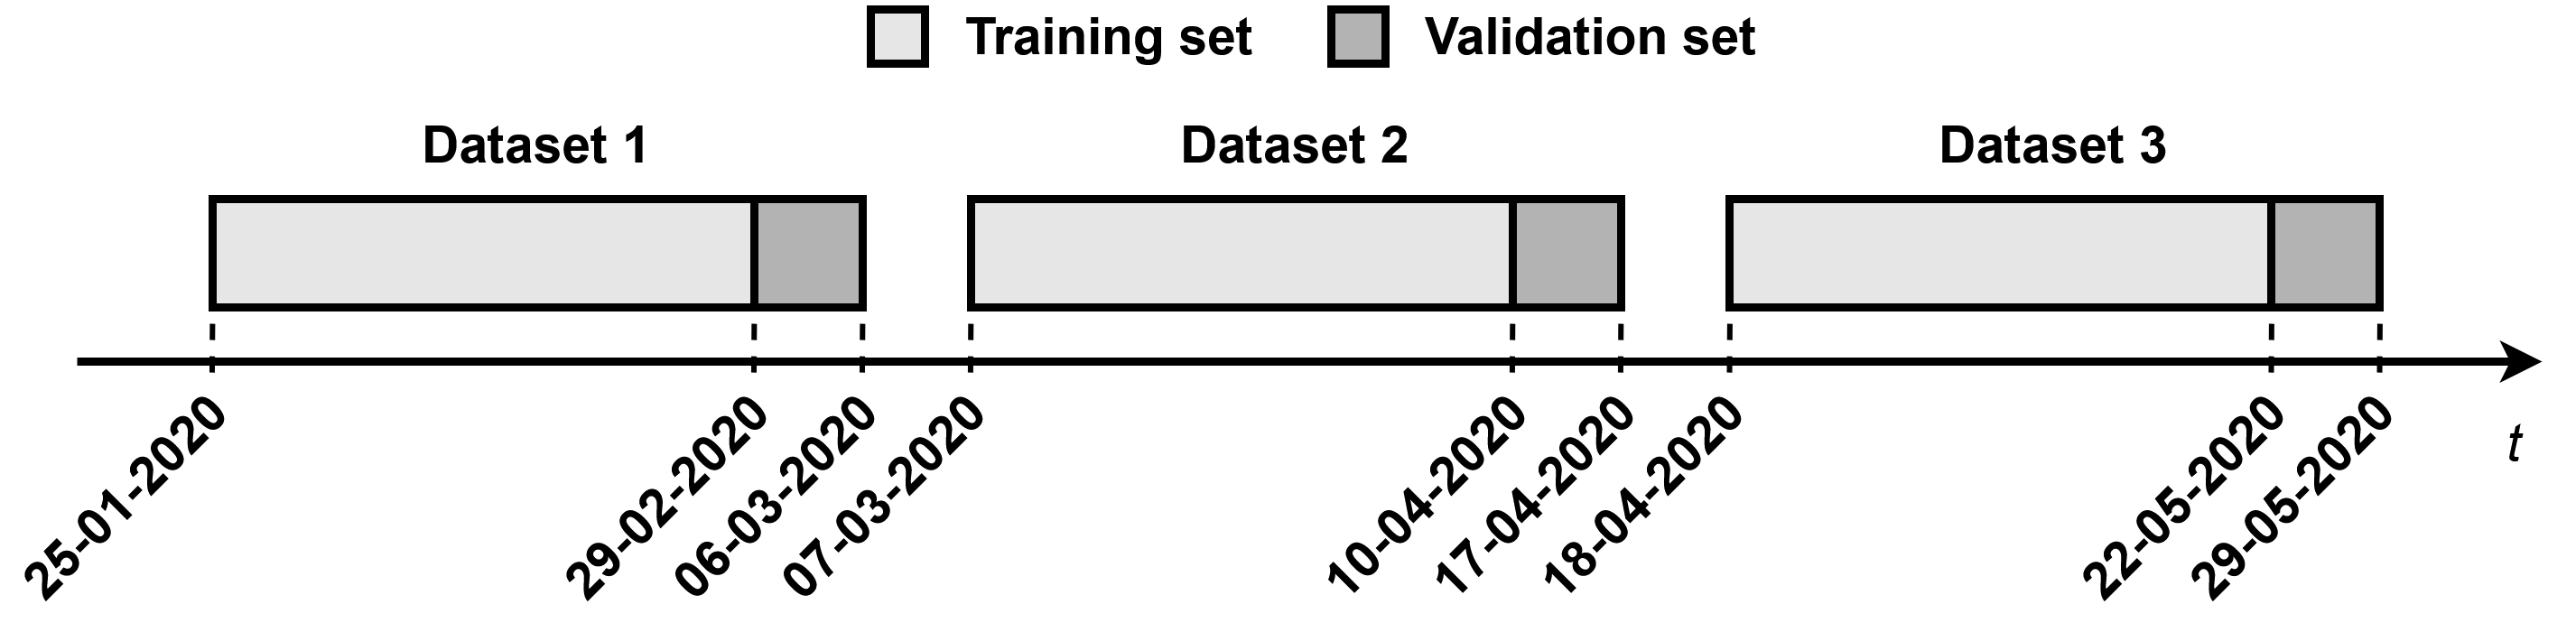
\includegraphics[width=1\textwidth]{Images/hyptun.png}
    \caption{Datasets used for expanding window cross-validation.}
    \label{hyptun}
    \end{center}
\end{figure}

The process of tuning hyperparameters is a long and time consuming process. Although the meaning of each hyperparameter and what it represents in the context of the layer is known, there is no rule dictating which hyperparamters are best for each case. It is an experimental process in which the models must be trained, and validated. The results obtained in the validation data are then compared for different hyperparameter combinations. The combination that presents the best results for each model, must be the one selected. To speed up this process, a script \cite{} was created, responsible for training and validating multiple combinations of hyperparameters for each of the proposed models. In total, about 84 different combinations were tested in each of the four blocks. Based on the results obtained in each block for each of the 84 combinations, the ideal hyperparameter combination for each of the six proposed models is defined, being the one that, on average, presents a lower error value in the four cases. In Appendix XXXX, one can find the tables with the validation errors registered for each of the four blocks.

As explained earlier, exhaustive grid-search was then used to test various combinations of hyperparameters for each of the models. In the layers \ac{GRU} and \ac{LSTM}, the number of units of each layer was consecutively changed.
The number of units is a positive integer that represents the dimensionality of the output space of the layer. This hyperparameter must be tuned in to find a value for which the system performs well. However, the increase of this value represents an increase in the complexity of the model, which makes it slower. Regarding the \ac{1D CNN} layers, the hyperparameters that were tested were the number of filters - An integer that represents dimensionality of the output space (i.e. the number of output filters in the convolution), the kernel\_size - An integer specifying the length of the 1D convolution window used. In the Max pooling layer, a pool\_size was fixed to 2 units, which means that only the highest value every 2 values is taken into account, as explained in the section \ref{chap3:subsubsec:1dcnn}. In order to avoid overfitting, dropout layers with $p=0.2$ were also used.

Another hyperparameter that is common to all architectures is the dimension of the sequences introduced at the entry-level, that is, how many steps back will the model have access to perform its predictions. For this we tested several options, for example, 15 steps back (i.e. use the last 15 minutes data to predict the next 15 minutes), 60 steps back (i.e. use the last hour data to predict the next 15 minutes), and 420 steps back (i.e. use the last seven hours data to predict the next 15 minutes).  Longer time windows have also been tested, but the conclusion is that increasing this value brings more disadvantages than advantages, namely in the training time of the model. In addition, since it is intended to predict in the very short term, the influence that data collected a week ago may have on the energy behavior of the building is quite small. It is also relevant to mention that the high granularity of the data used (1 minute), quickly turns the training process of any model very slow when using very large time windows. For example, if one wants to use the data of the last week, to predict a single iteration of 15 steps, it is necessary to use 60*24*7 = 10080 steps of the past which, in practice, can quickly become quite demanding computationally. Among the three options presented, it was chosen to use the second one, where data from the last hour is used to predict the next 15 minutes. The difference in performance obtained by each of the models compared to the third option (420 steps), did not present drastic changes that would compensate the choice of the most expensive option. Compared to the past 15 steps, the use of 60 steps showed some improvements, so the second option was chosen. It is important to point out that the purpose of this choice comes from the nature of the data and the goals of the case study in question. However, it may be developed in future work the use not only of more values from the past for the production of each iteration, but also the modification of the granularity of the data used.

For each of the four blocks defined in the expanding window cross-validation process, the architectures were trained and validated. The hyperarameters already mentioned were progressively optimized in the four blocks, for each model. As we know, the motivation behind this step is only to compare the different sets of hyperparameters used in each of the models, and not to compare the different models among themselves. This comparison is only done later, when the chosen models are tested in the Test set. In Table \ref{valres}, the reader may consult the results of the expanding window cross-validation process, which consists of an average of the errors presented in blocks 1, 2, 3 and 4.

% Table generated by Excel2LaTeX from sheet 'Tabel Creation'
\begin{table}[htbp]
  \centering
  \caption{Selected models resulting from window cross-validation procedure.}
    \begin{tabular}{r|c|cc|cccc}
    \multicolumn{1}{c|}{\multirow{2}[0]{*}{\textbf{Model}}} & \multirow{2}[0]{*}{\textbf{Naïve}} & \multicolumn{2}{c|}{\textbf{Vanilla}} & \multicolumn{1}{l}{\textbf{Encoder-Decoder}} &   &   &  \\
      &   & GRU & LSTM & GRU-GRU & LSTM-LSTM & CNN-GRU & CNN-LSTM \\
    \# inputs & - & 13 & 13 & 13 & 13 & 13 & 13 \\
    \# hidden layers & - & 1 & 1 & - & - & - & - \\
    \# hidden nodes & - & 256 & 256 & - & - & - & - \\
    \# encoder nodes & - & - & - & 16 & 64 & 16 & 64 \\
    \# decoder nodes & - & - & - & 16 & 64 & 64 & 64 \\
    \midrule
    \textbf{Validation (t+5)} &   &   &   &   &   &   &  \\
    RMSE (E-02) & 2.674 & 2.559 & 2.684 & 2.684 & 2.695 & 3.089 & 3.194 \\
    MSE(E-03) & 0.716 & 0.656 & 0.724 & 0.721 & 0.729 & 0.960 & 1.021 \\
    MAE (E-02) & 1.891 & 1.840 & 1.962 & 2.054 & 2.022 & 2.327 & 2.466 \\
    \textbf{Validation (t+10)} &   &   &   &   &   &   &  \\
    RMSE (E-02) & 3.118 & 3.014 & 3.162 & 3.067 & 3.042 & 3.432 & 3.458 \\
    MSE(E-03) & 0.973 & 0.910 & 1.008 & 0.941 & 0.927 & 1.182 & 1.196 \\
    MAE (E-02) & 2.247 & 2.185 & 2.302 & 2.324 & 2.270 & 2.588 & 2.653 \\
    \textbf{Validation (t+15)} &   &   &   &   &   &   &  \\
    RMSE (E-02) & 3.458 & 3.351 & 3.477 & 3.343 & 3.348 & 3.743 & 3.730 \\
    MSE(E-03) & 1.197 & 1.125 & 1.214 & 1.118 & 1.123 & 1.404 & 1.392 \\
    MAE (E-02) & 2.517 & 2.437 & 2.542 & 2.510 & 2.498 & 2.828 & 2.858 \\
    \midrule
    \textbf{Total Validation} &   &   &   &   &   &   &  \\
    RMSE (E-02) & 3.083 & 2.975 & 3.108 & 3.032 & 3.028 & 3.421 & 3.461 \\
    MSE(E-03) & 0.962 & 0.897 & 0.982 & 0.927 & 0.926 & 1.182 & 1.203 \\
    MAE (E-02) & 2.219 & 2.154 & 2.269 & 2.296 & 2.263 & 2.581 & 2.659 \\
    \end{tabular}%
  \label{valres}%
\end{table}%

Table \ref{valres} is divided into three parts, and summarizes the information regarding the best set of hyperparameters for each of the six models. In the first part, some important factors related to the general architecture of the sectioned models can be seen. The number of inputs, equal for the six models, is presented, which refers to the number of features defined in the \ac{PCA} process described in section \ref{chap3:subsec:feature_selection}, the number of hidden layers and hidden nodes, which was only considered in the Vanilla architectures, and the number of encoder and decoder nodes, only considered in the Encoder-Decoder architectures. In the second part of the table, the \ac{MSE}, \ac{RMSE} and \ac{MAE} validation values are presented for each one of the models, which refers to the forecast of the available power in 5, 10 and 15 minutes. All these values are an average of the results obtained for each of the four blocks, as defined in section \ref{chap3:subsec:data_partition}. It should be noted that, the two Vanilla models produce only 3 values, due to the nature of many-to-one models. On the other hand, the remaining models, many-to-many, produce whole sequences with 15 values. For the first two models, the errors shown in Table \ref{valres}  result from direct comparison between the first value produced by the model and the actual power available in 5 minutes, a process that is equally valid for the other two metrics. For the Encoder-Decoder models, the errors were calculated by comparing the fifth value of the sequence generated by the model, with the fifth value of the measured sequence for the same time-interval, and so on for the remaining two readings. The third and last part of Table \ref{valres} corresponds to the average value of each metric for the three time intervals. It was decided to determine this value to enable the global evaluation of each of the models, and not just the individual evaluation for each one of the time targets. With these average metrics, it is then possible to compare the performance of models at a global scale.


When reviewing the data in Table \ref{valres}, it is quite easy to incur in the mistake of trying to compare the results obtained by each of the models with each other. However, one must remember that the metrics described in the table are the results of the validation process and not the test. Although some estimates of the true performance of the models can be drawn from these results, to evaluate their performance fairly and properly, it is necessary to use a set of data never seen before, the Test set, where the model can be tested in an unbiased environment. This procedure is described in Stage 2.


\section{Stage 2 - Results}\label{chap3:section:stage_2}

In the previous step, the combination of hyperparameters, for each one of the models, that presented the best performance overall was defined. In this stage, the six models are re-trained in all the available training data, which consists of training the models in the whole block 4 and testing their performance in the test data. In Figure \ref{test} the reader can find a graphic representation of this process.

\begin{figure}[h!]
    \centering
    \begin{center}
    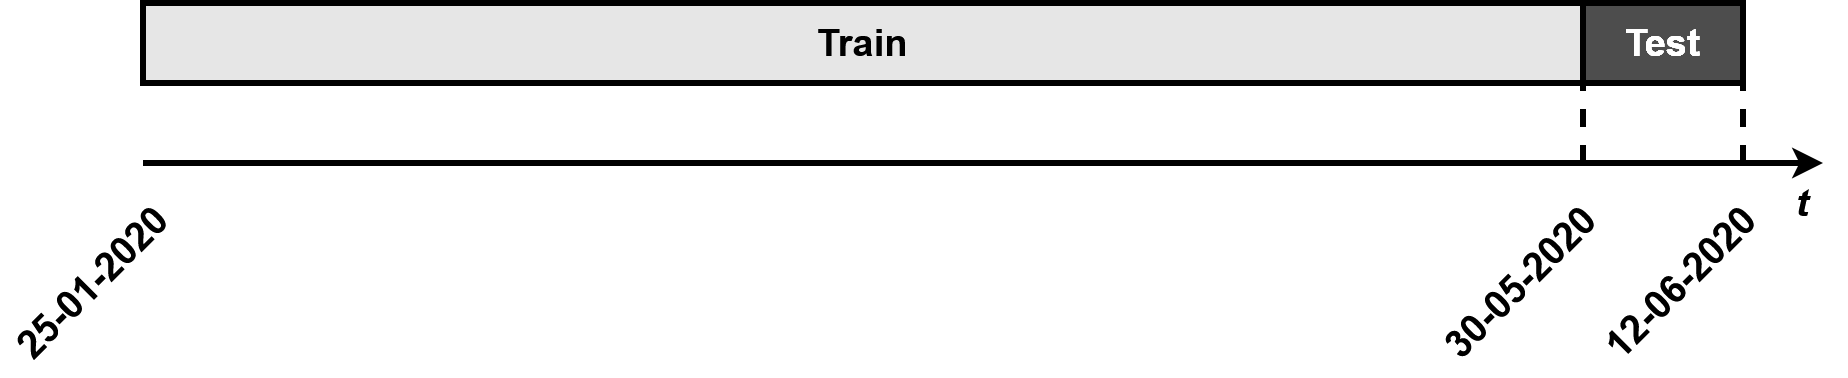
\includegraphics[width=1\textwidth]{Images/test2.png}
    \caption{Dataset used for testing the final models.}
    \label{test}
    \end{center}
\end{figure}

Table XX shows the results of the test process where the 6 models were tested. It is also possible to observe the results obtained when applying the Naive Model in the test set. These values act as a comparative basis of the results obtained by the remaining models.

\begin{table}[htbp]
  \centering
  \caption{Add caption}
    \begin{tabular}{r|c|cc|cccc}
    \multicolumn{1}{c|}{\multirow{2}[1]{*}{\textbf{Model}}} & \multirow{2}[1]{*}{\textbf{Naïve}} & \multicolumn{2}{c|}{\textbf{Vanilla}} & \multicolumn{4}{c}{\textbf{Encoder-Decoder}} \\
      &   & GRU & LSTM & GRU-GRU & LSTM-LSTM & CNN-GRU & CNN-LSTM \\
    \midrule
    \textbf{Test (t+5)} &   &   &   &   &   &   &  \\
    RMSE (E-02) & 2.735 & 2.521 & 2.762 & 2.606 & 2.575 & 2.694 & 3.475 \\
    MSE(E-03) & 0.748 & 0.636 & 0.763 & 0.679 & 0.663 & 0.726 & 1.207 \\
    MAE (E-02) & 1.911 & 1.813 & 1.969 & 1.904 & 1.854 & 1.853 & 2.453 \\
    \textbf{Test (t+10)} &   &   &   &   &   &   &  \\
    RMSE (E-02) & 3.159 & 2.955 & 3.187 & 3.007 & 3.013 & 3.077 & 3.86 \\
    MSE(E-03) & 0.998 & 0.873 & 1.016 & 0.904 & 0.908 & 0.947 & 1.49 \\
    MAE (E-02) & 2.188 & 2.059 & 2.244 & 2.138 & 2.117 & 2.091 & 2.677 \\
    \textbf{Test (t+15)} &   &   &   &   &   &   &  \\
    RMSE (E-02) & 3.547 & 3.176 & 3.344 & 3.283 & 3.308 & 3.380 & 4.106 \\
    MSE(E-03) & 1.258 & 1.009 & 1.118 & 1.078 & 1.094 & 1.143 & 1.686 \\
    MAE (E-02) & 2.449 & 2.128 & 2.314 & 2.266 & 2.274 & 2.279 & 2.823 \\
    \midrule
    \textbf{Total Test} &   &   &   &   &   &   &  \\
    RMSE (E-02) & 3.147 & 2.884 & 3.098 & 2.965 & 2.965 & 3.051 & 3.814 \\
    MSE(E-03) & 1.001 & 0.839 & 0.966 & 0.887 & 0.888 & 0.938 & 1.461 \\
    MAE (E-02) & 2.182 & 2.000 & 2.176 & 2.103 & 2.082 & 2.074 & 2.651 \\
    \end{tabular}%
  \label{tab:addlabel}%
\end{table}%











\begin{figure}[h!]
\captionsetup[subfigure]{position=b}
\centering
\subcaptionbox{\label{m1}}{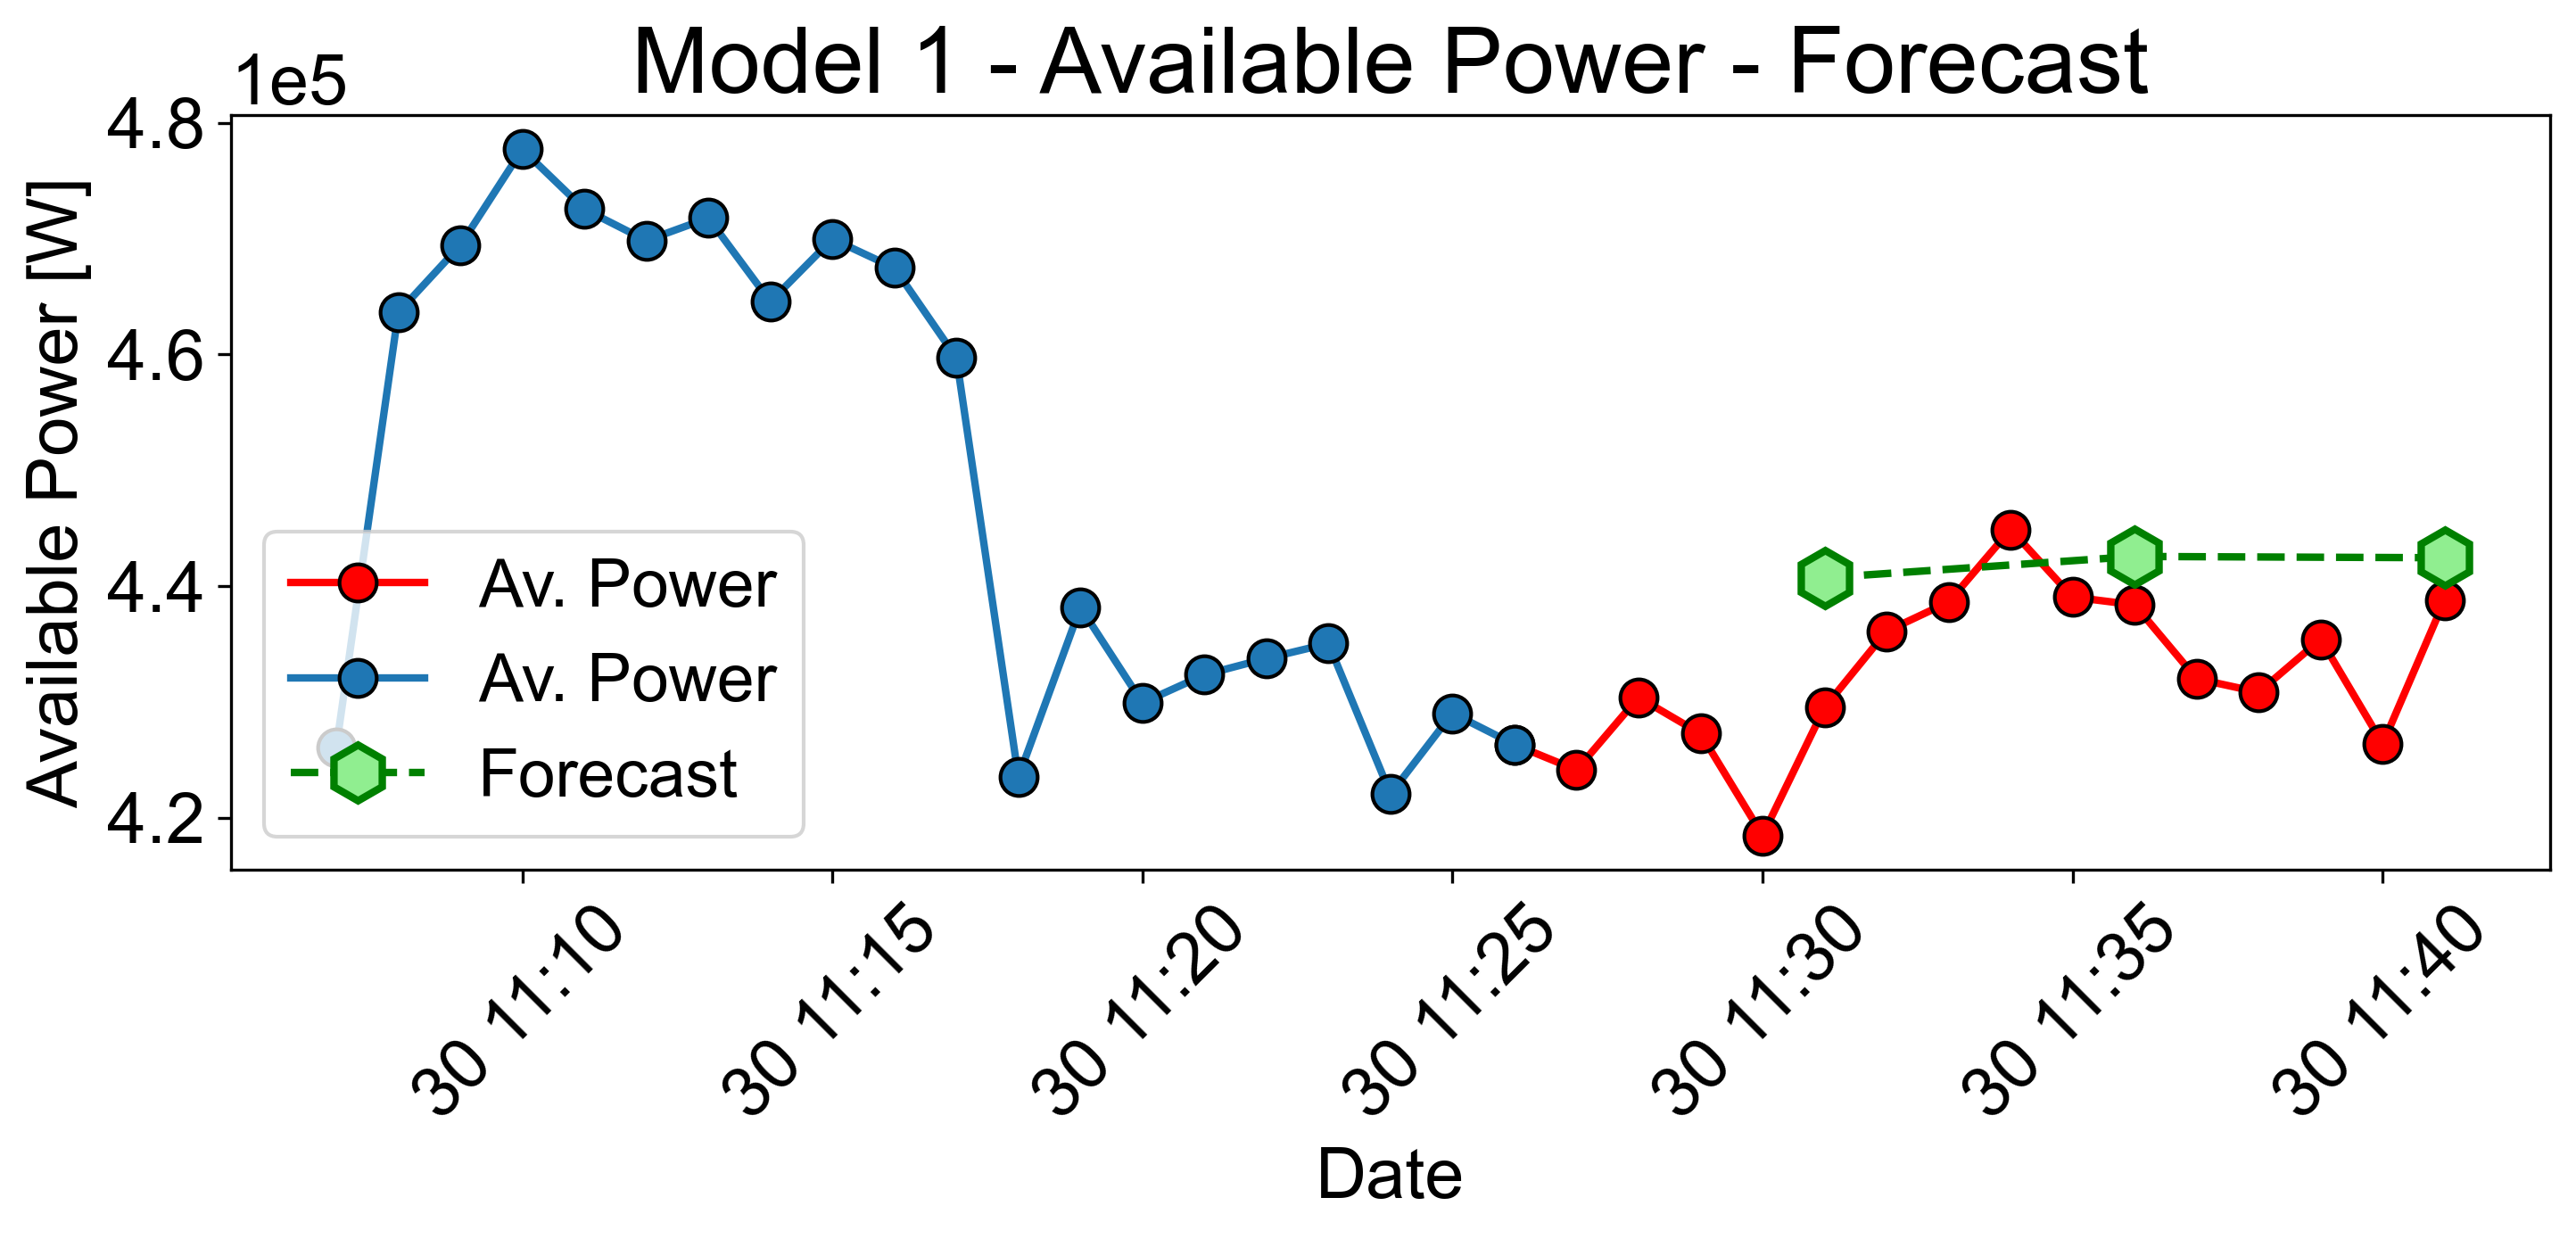
\includegraphics[width=.49\linewidth]{Images/F1-GRU-16.png}}
\subcaptionbox{\label{m2}}{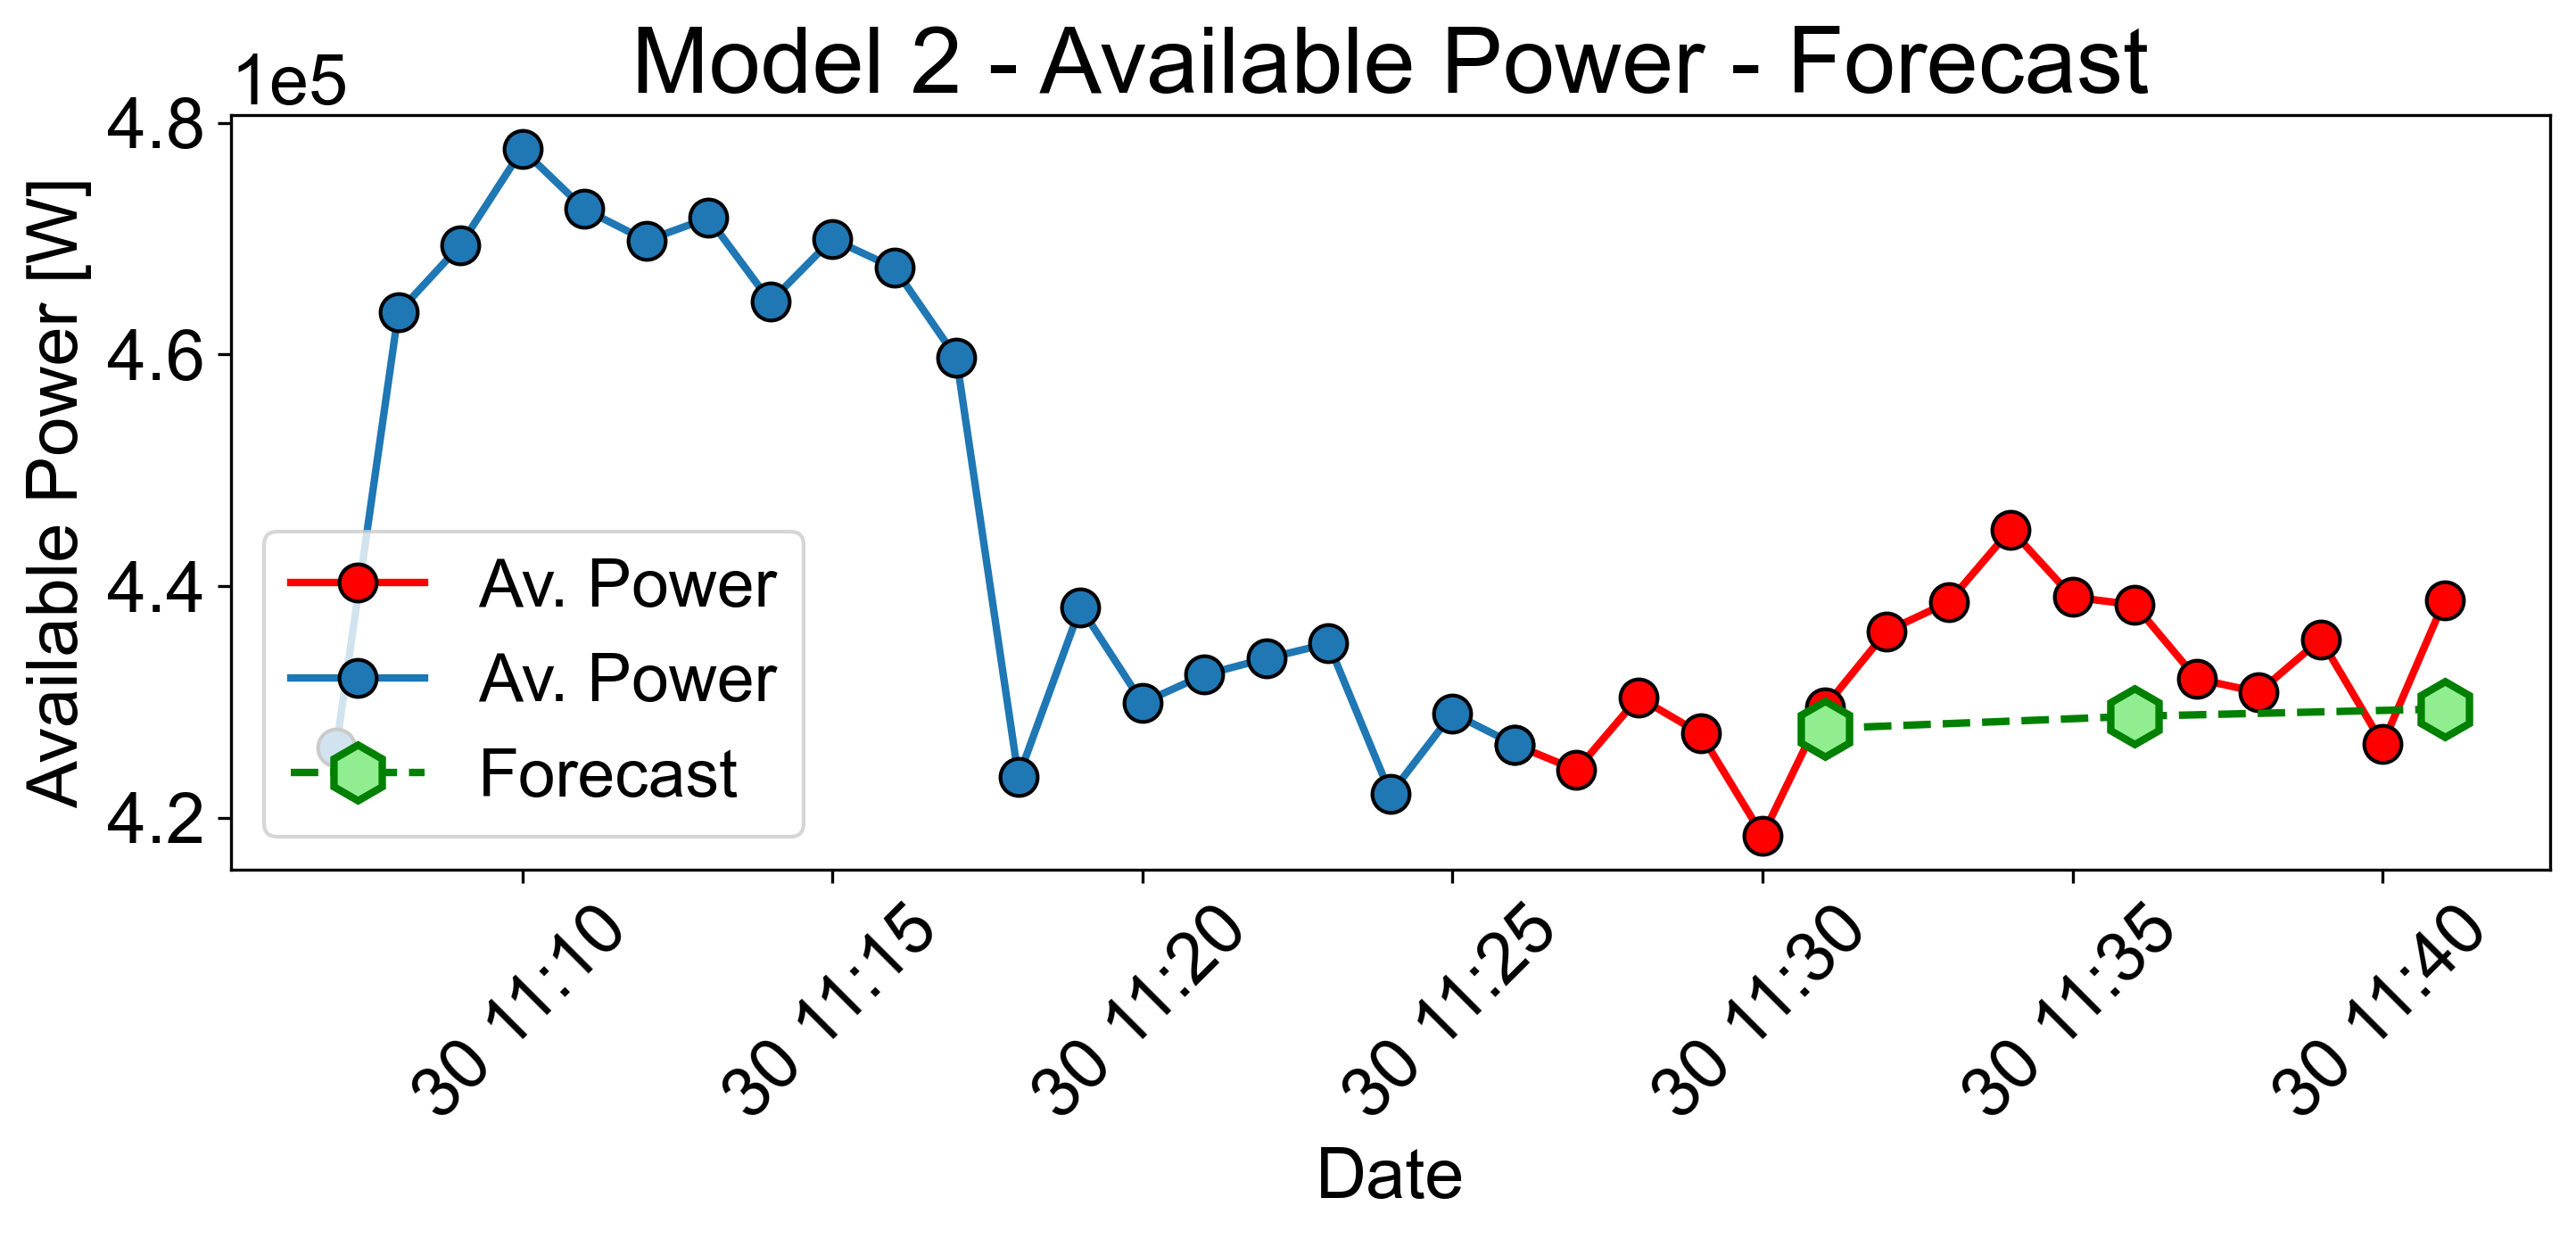
\includegraphics[width=.49\linewidth]{Images/F2-LSTM-16.png}}

\subcaptionbox{\label{m3}}{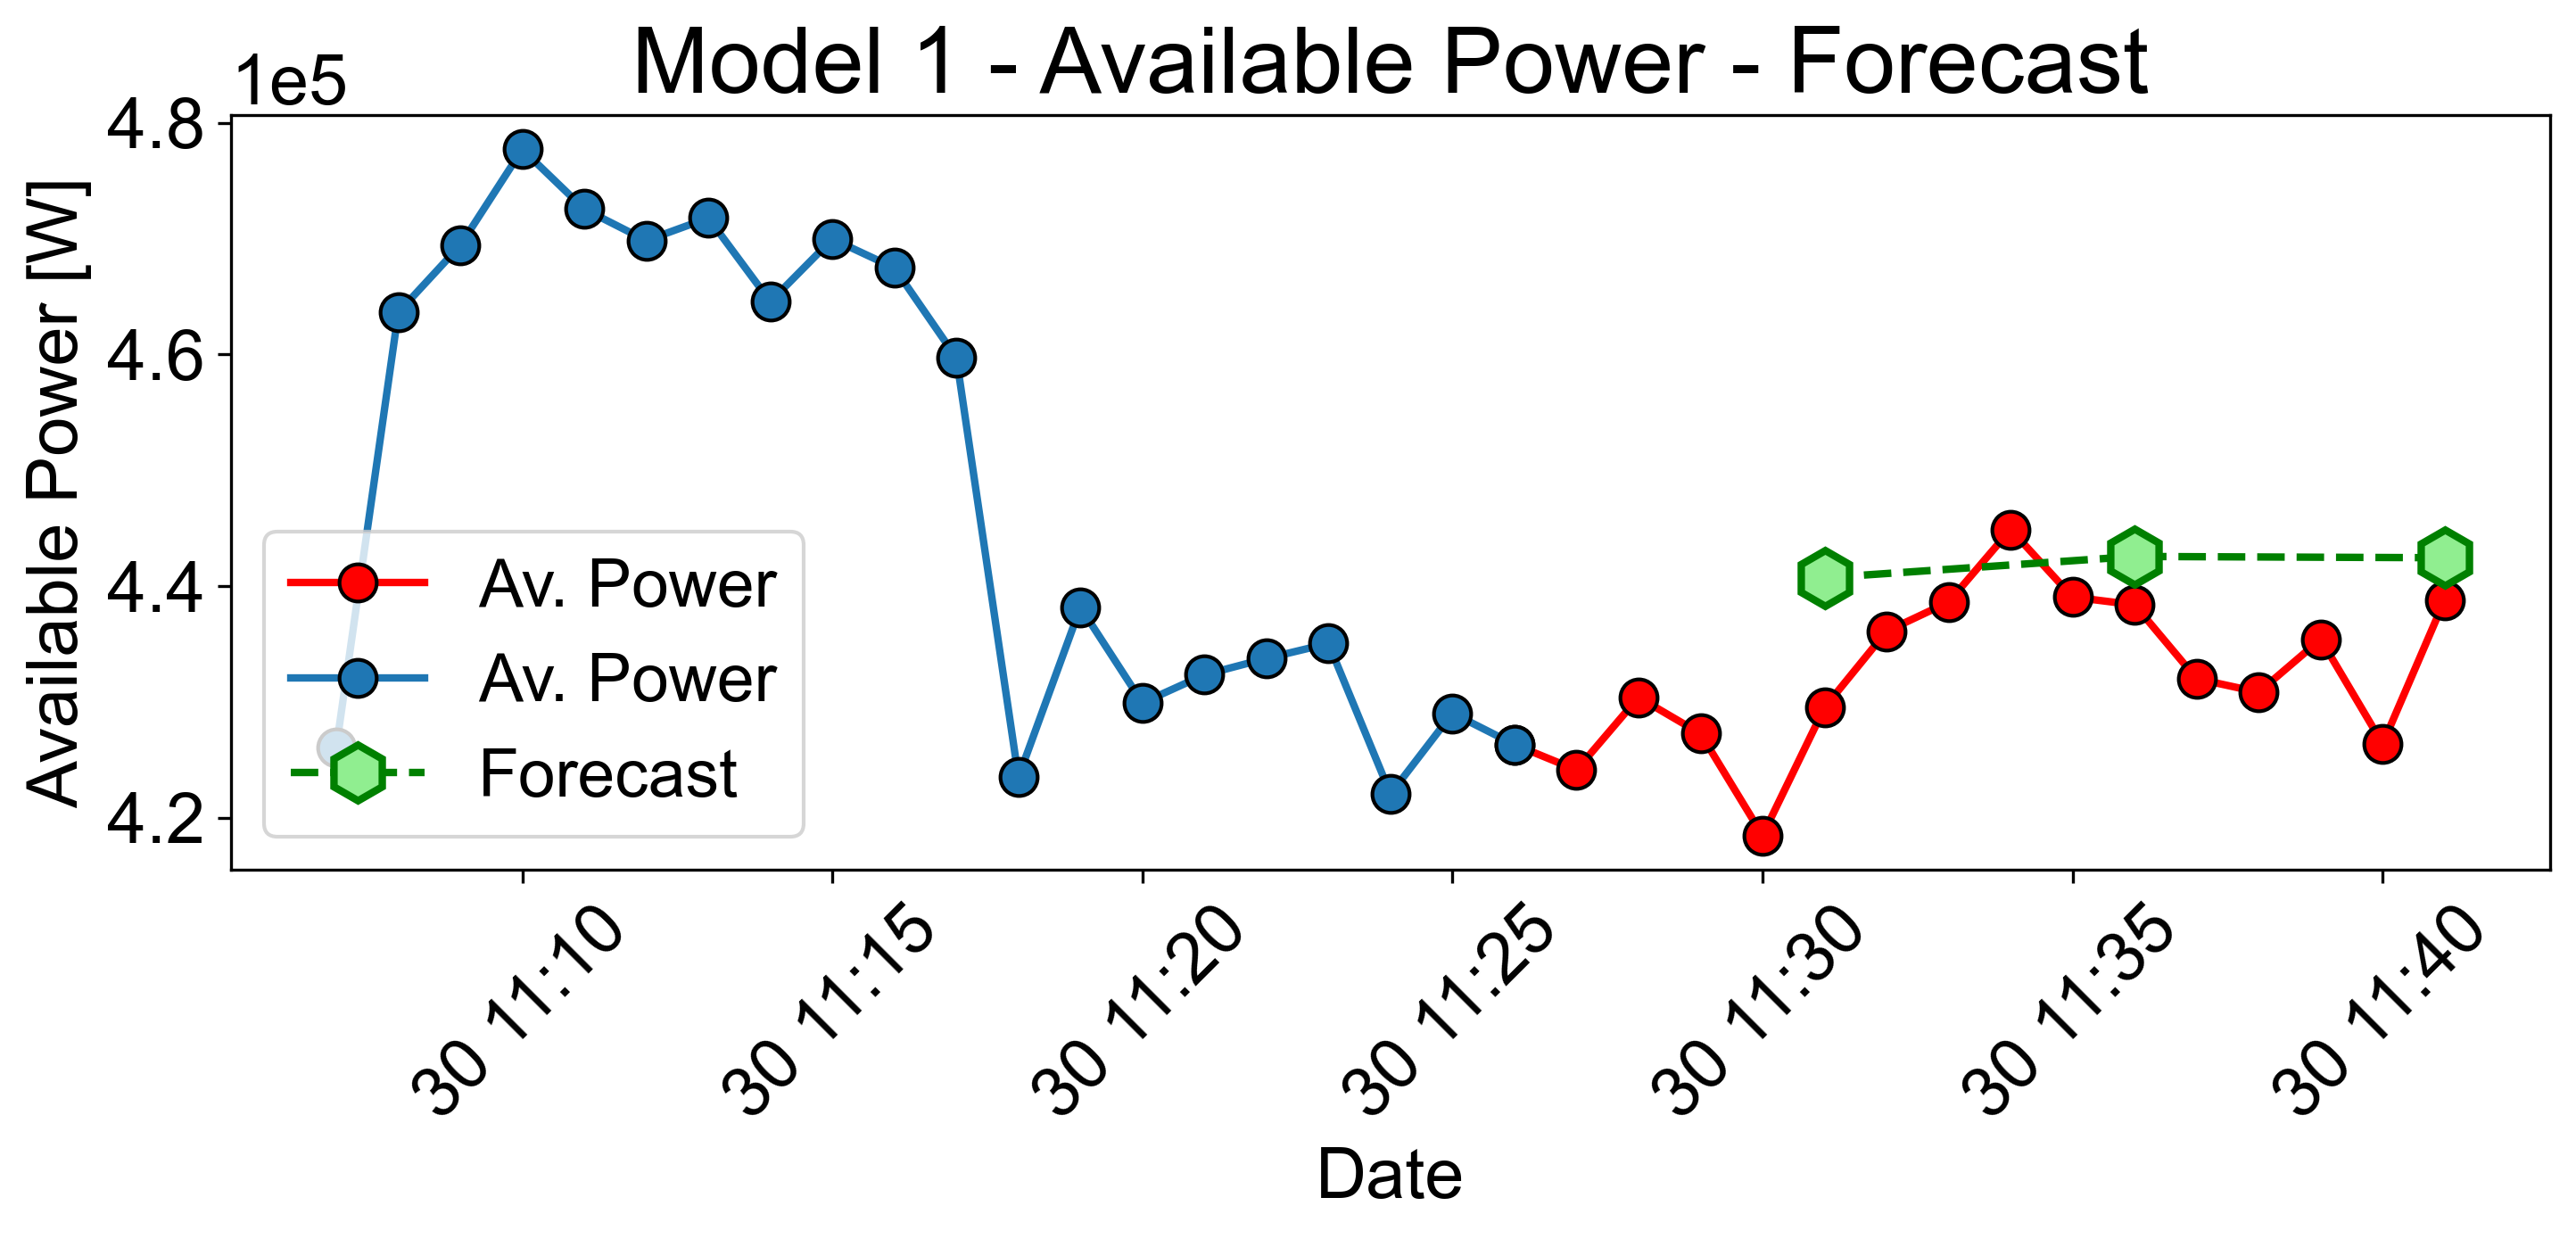
\includegraphics[width=.49\linewidth]{Images/F1-GRU-16.png}}
\subcaptionbox{\label{m4}}{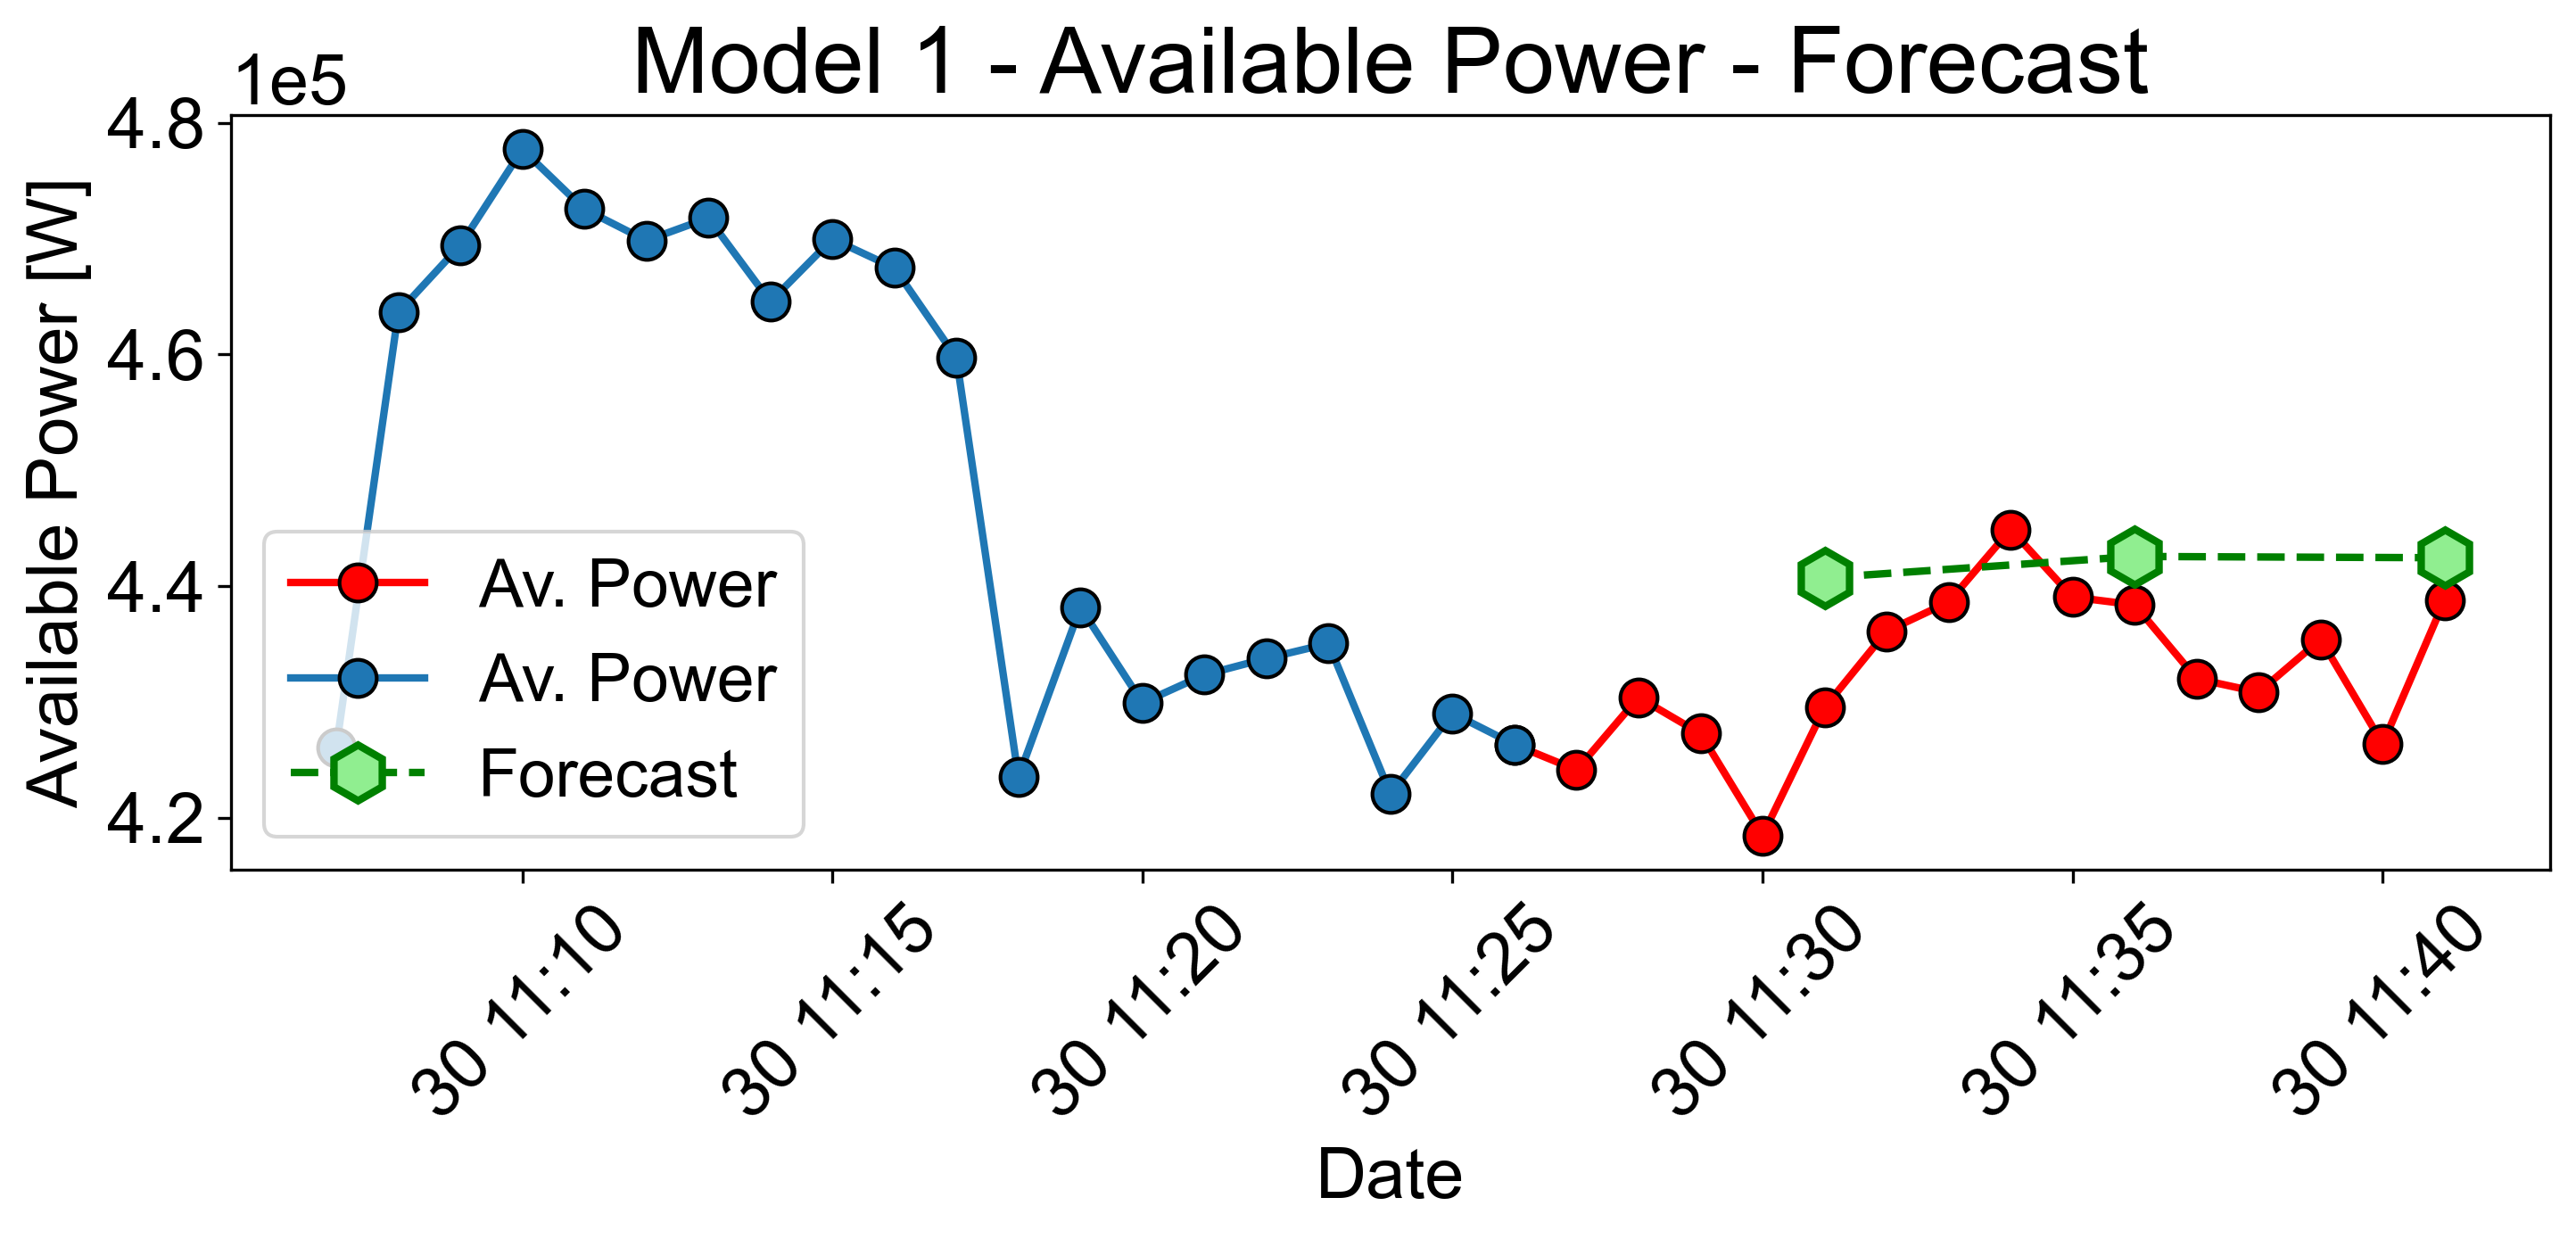
\includegraphics[width=.49\linewidth]{Images/F1-GRU-16.png}}

\subcaptionbox{\label{m5}}{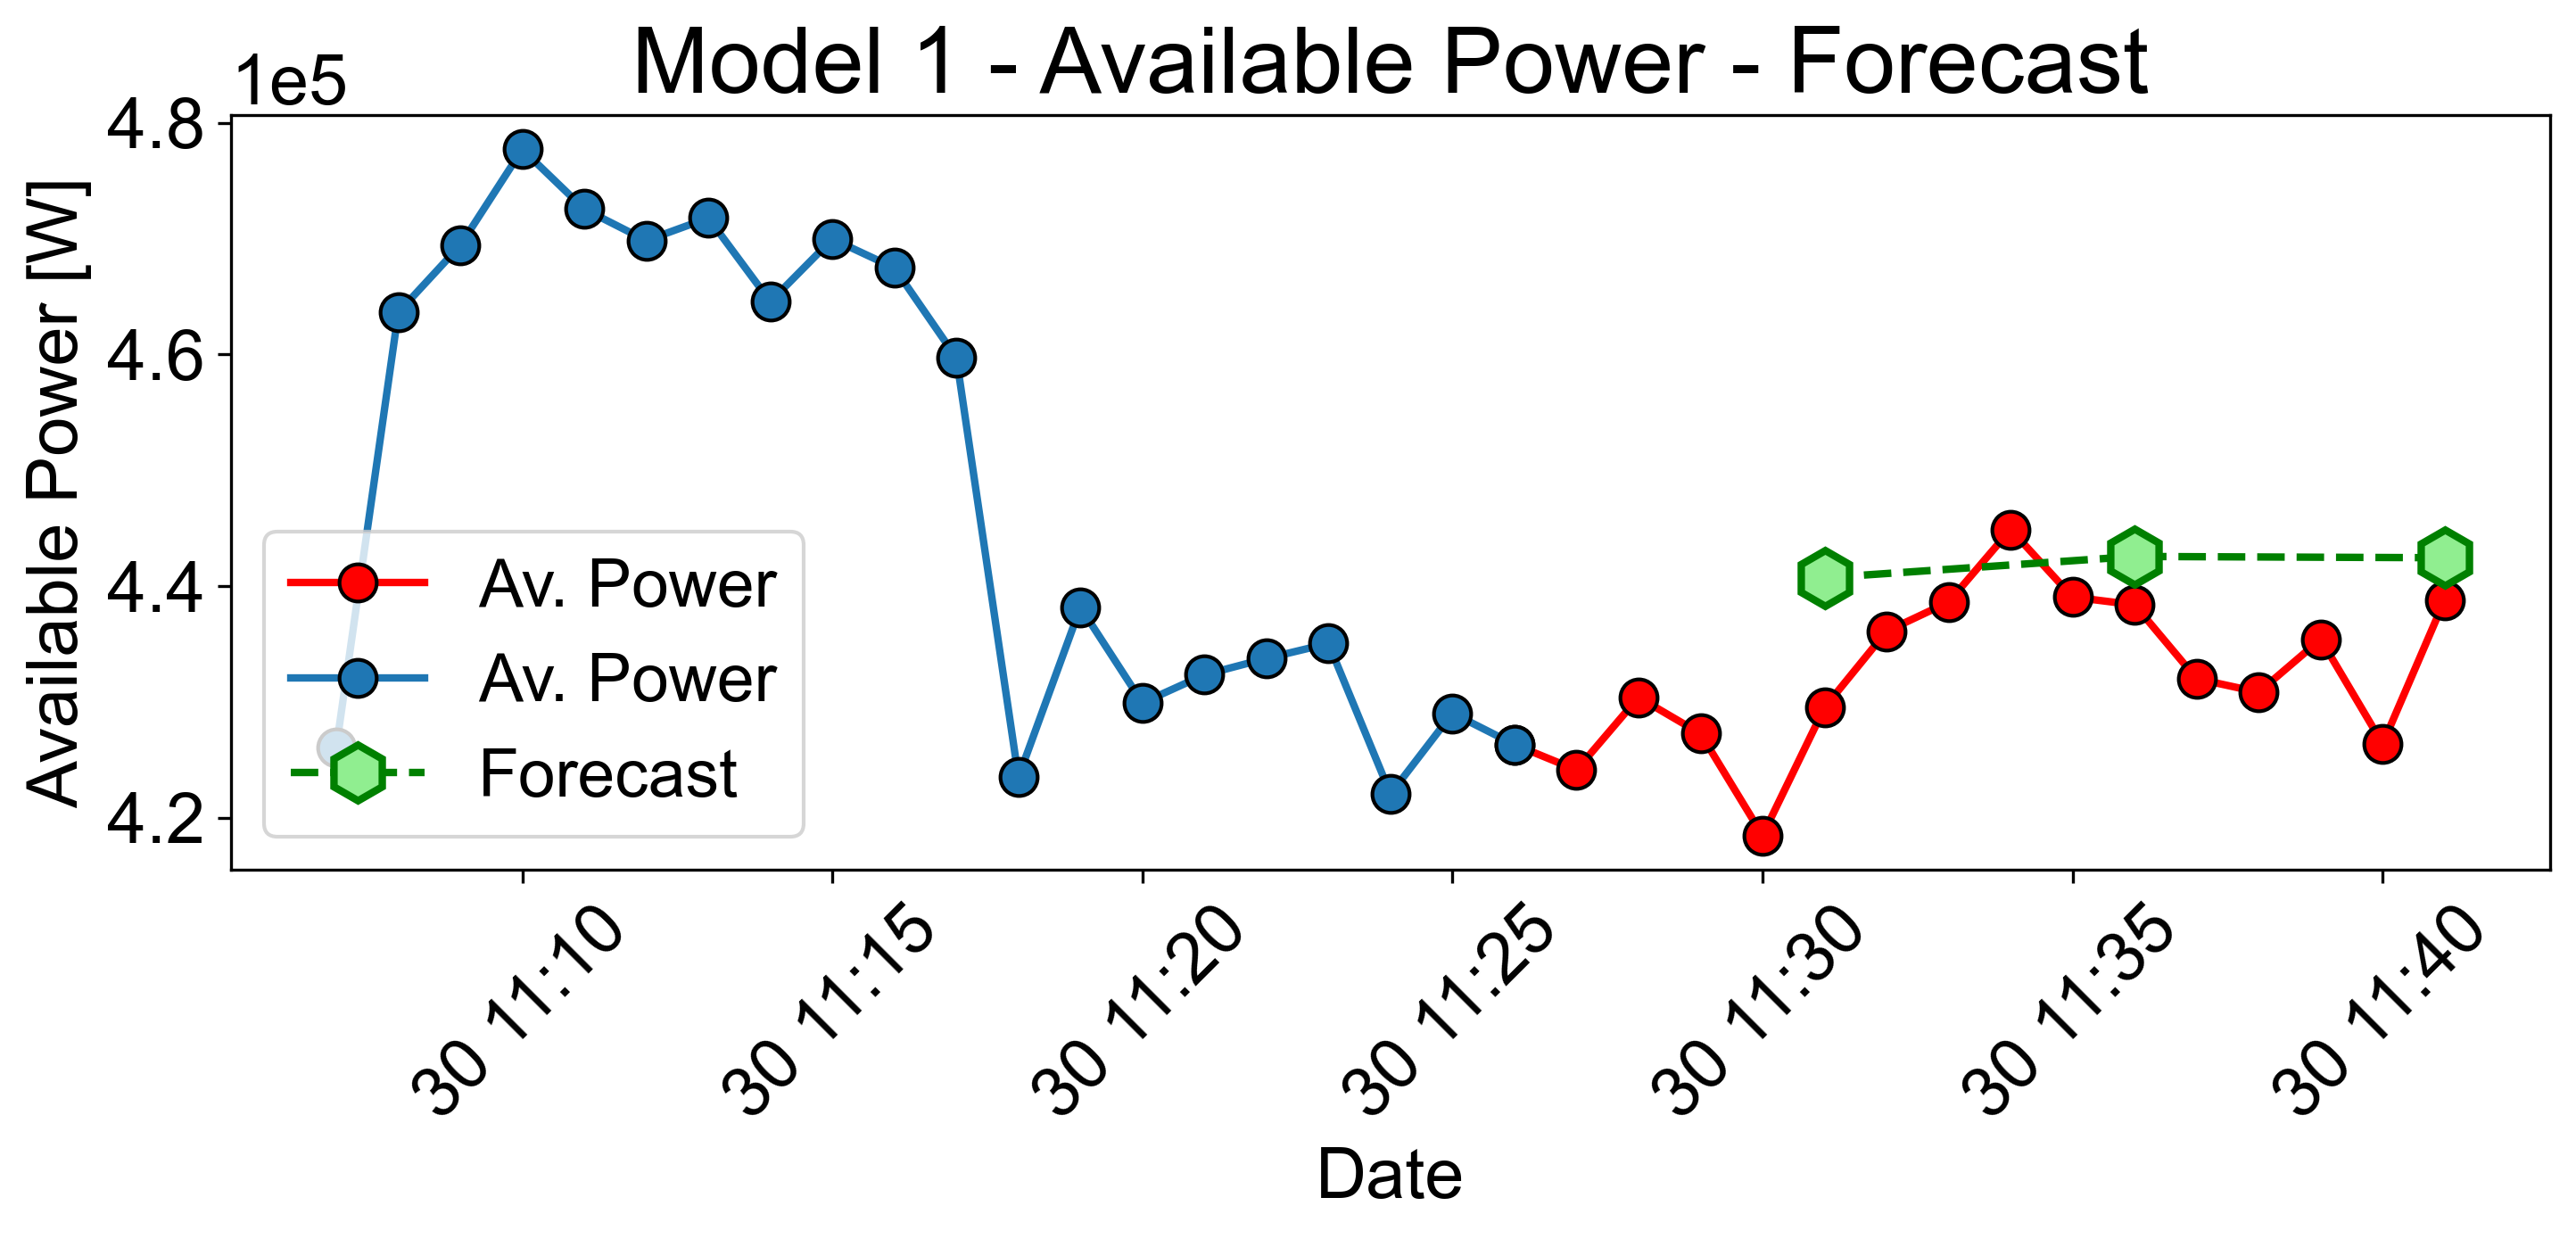
\includegraphics[width=.49\linewidth]{Images/F1-GRU-16.png}}
\subcaptionbox{\label{m6}}{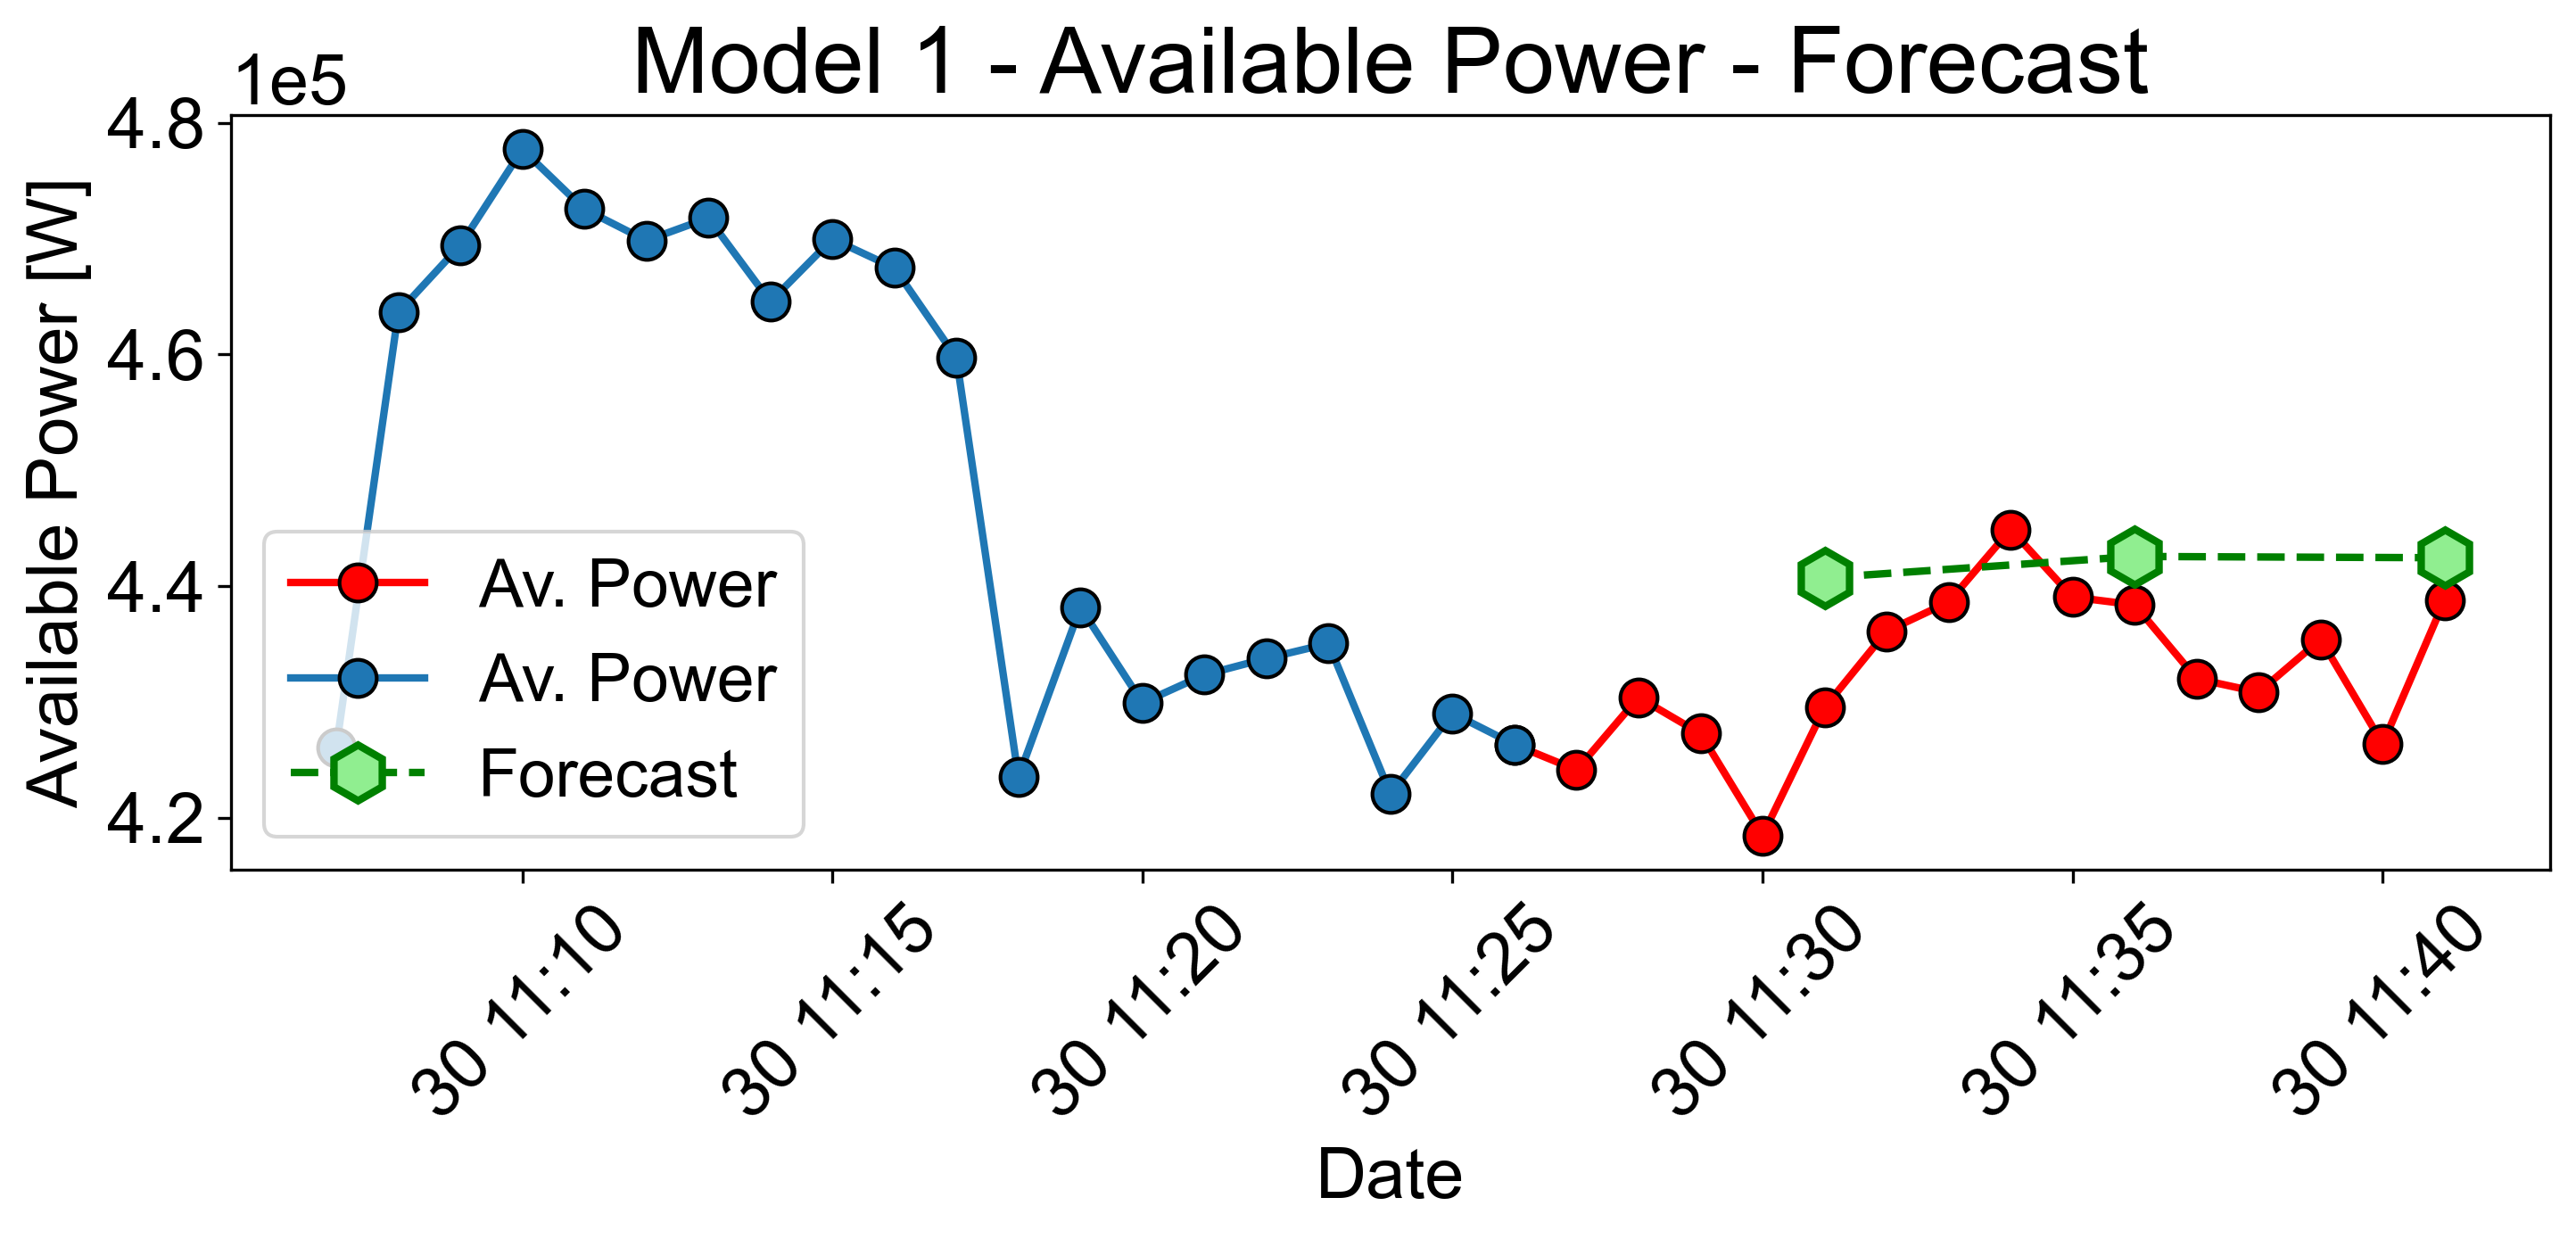
\includegraphics[width=.49\linewidth]{Images/F1-GRU-16.png}}
\caption{Example data a) Before convolution b) after convolution c) after Max pooling.}
\label{resgra}
\end{figure}










\newpage
\section{Stage 3 - Confidence intervals}\label{chap3:section:stage_3}

It is true that the main goal is to set a value for the available power at 5, 10 and 15 minutes, but it would be interesting to set a maximum and a minimum value for each of these three forecasts. In other words, it would be important to be able to project a confidence interval of the forecasts carried out. 

In order to project the confidence interval of a forecast from a set of points $x(t, ..., N)$, multiple sets of values are needed for this interval, that is, based on the same input data, the model would have to be able to generate several forecast values for this instant, but this does not happen. As we know, \ac{ANNs}, after the training process in which the weights are defined, become deterministic functions, which means that for the same input, the same predicted output will always be produced, regardless of the number of times the algorithm runs. We are then faced with a limitation, the impossibility of obtaining several values for the same instant, so that a confidence interval of the forecast can be computed.

In 2017, Zhu proposed a technique to solve this problem \cite{uber}. The principle is to adapt the predictive model so that it can return multiple (different) predictions by applying dropout in the forecast process. As discussed in section \ref{chap3:subsubsec:regularization_techniques}, one of the most common techniques to avoid overfitting is the use of dropout layers. Usually, these layers are active in the training process, in order to introduce some error in the model to prevent it from overadapting to the data provided. But in the testing phase, these layers are disabled. The application of dropout "turns off" a randomly chosen fraction of the units of the model. Applying dropout in the testing process would imply that the model ceases to be deterministic, that is, for the same input, different outputs are generated each time forecasts are made. 
This principle is also known as \ac{MCD} \cite{uber2}, which dictates that the uncertainty of the model can be estimated by sample variance of the forecasts of the adapted model in some repetitions. For example, if for each input sequence, 100 distinct output sequences are predicted, assuming the dropout is maintained, all 100 sequences are different. By averaging the 100 sequences, one obtains an average forecast of the model, which can be assumed to be the actual result of the model forecast, that can be called MC Dropout Forecast. On the other hand, since for each instant you have 100 different values, the standard deviation of the 100 values can then be used to calculate the confidence interval of each of the values and, ultimately, the complete sequence. Assuming that the forecasts have a normal distribution $N(\mu, \sigma^2)$, with a mean $\mu$ and a standard deviation $\sigma$, it is then possible to determine the confidence intervals given by: 

\begin{equation}
    [\hat{y}^* - z_{\frac{\alpha}{2}}\mu,\ \hat{y}^* + z_{\frac{\alpha}{2}}\mu], 
\end{equation}

where $\hat{y}^* = \frac{1}{B}\sum_{b=1}^B\hat{y_b}$, and $\mu = \sqrt{\frac{1}{B}\sum_{b=1}^B(\hat{y_b} -\hat{y}^*)^2}$. In order to to compute the 95\% confidence interval, for example, the parameters should be $\alpha=0.05$ and $z_{\frac{\alpha}{2}}= 1.92$ . 

Another consideration that should be made is the selection of the parameter $p$ in the MC dropout. If the MC dropout is too large, the forecasts generated will be quite sparse, which in turn implies that the confidence intervals created will be too large. On the other hand, if the MC dropout is too small, the forecasts made will be too similar to each other, which results in very small confidence intervals. When $p$ value is ideal, there is an almost perfect correspondence between the confidence interval and the values obtained. For the problem in question, the parameter $p$ of the MC dropout was tested for various values, and it was concluded that a good value would again be $p = 0.2$.

In Figure \ref{mtcdrop} we can see the results of applying the \ac{MCD} method.

\begin{figure}[h!]
\captionsetup[subfigure]{position=b}
\centering
\subcaptionbox{\label{mc1}}{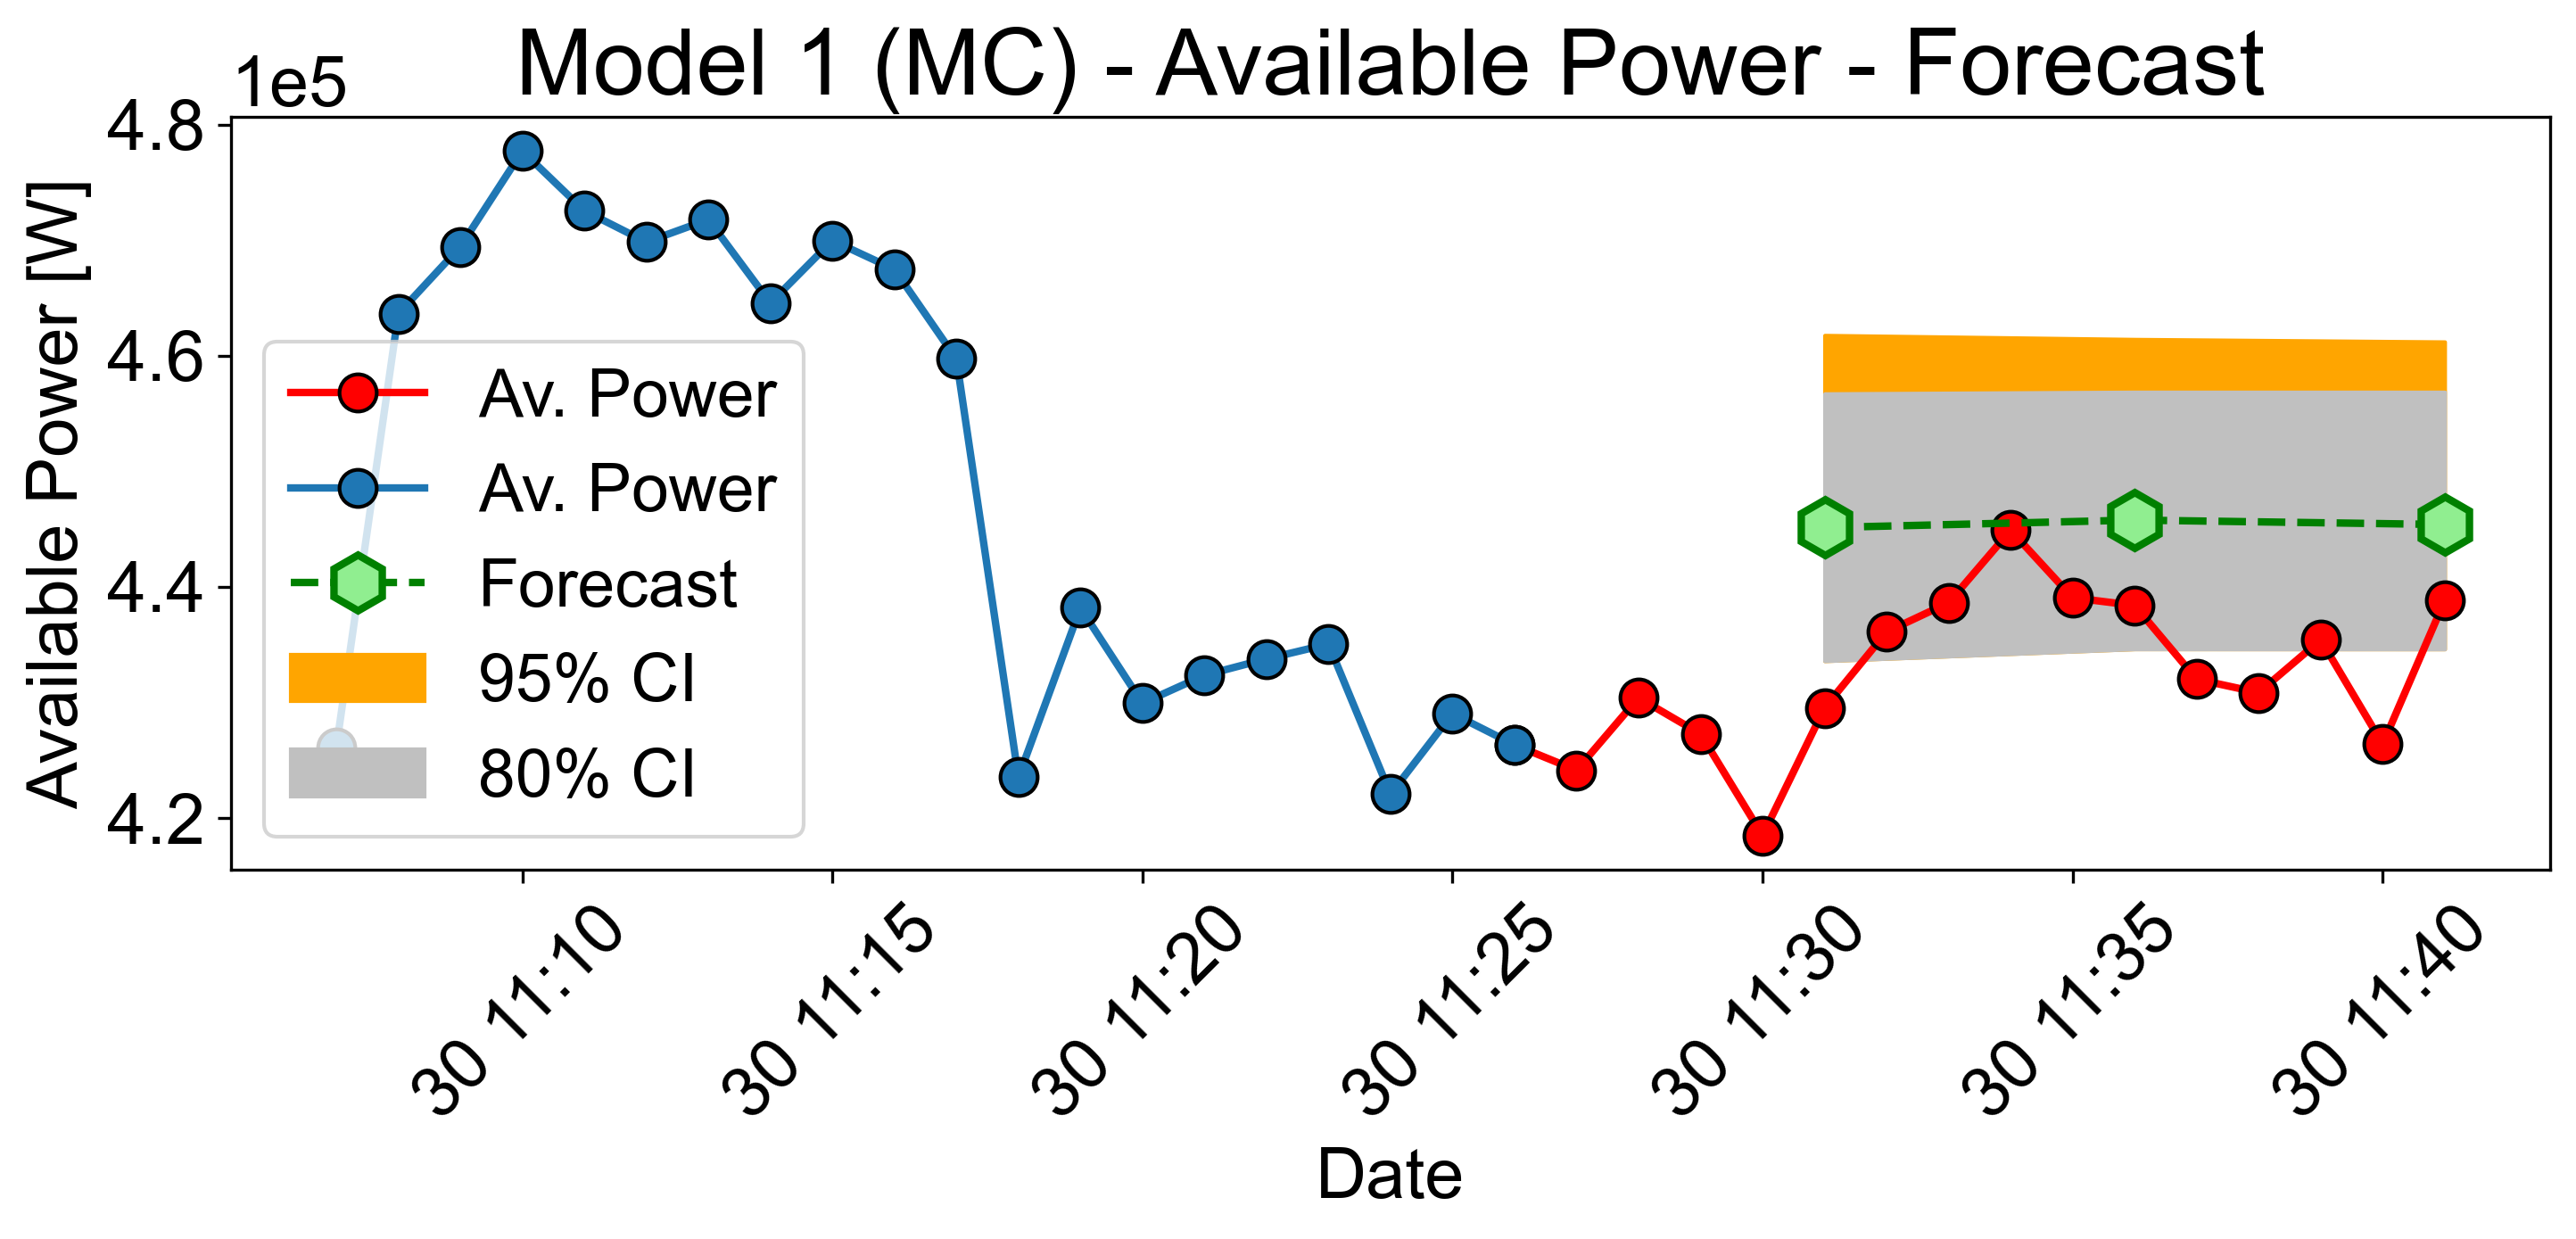
\includegraphics[width=.49\linewidth]{Images/MC-F1-GRU-16.png}}
\subcaptionbox{\label{mc2}}{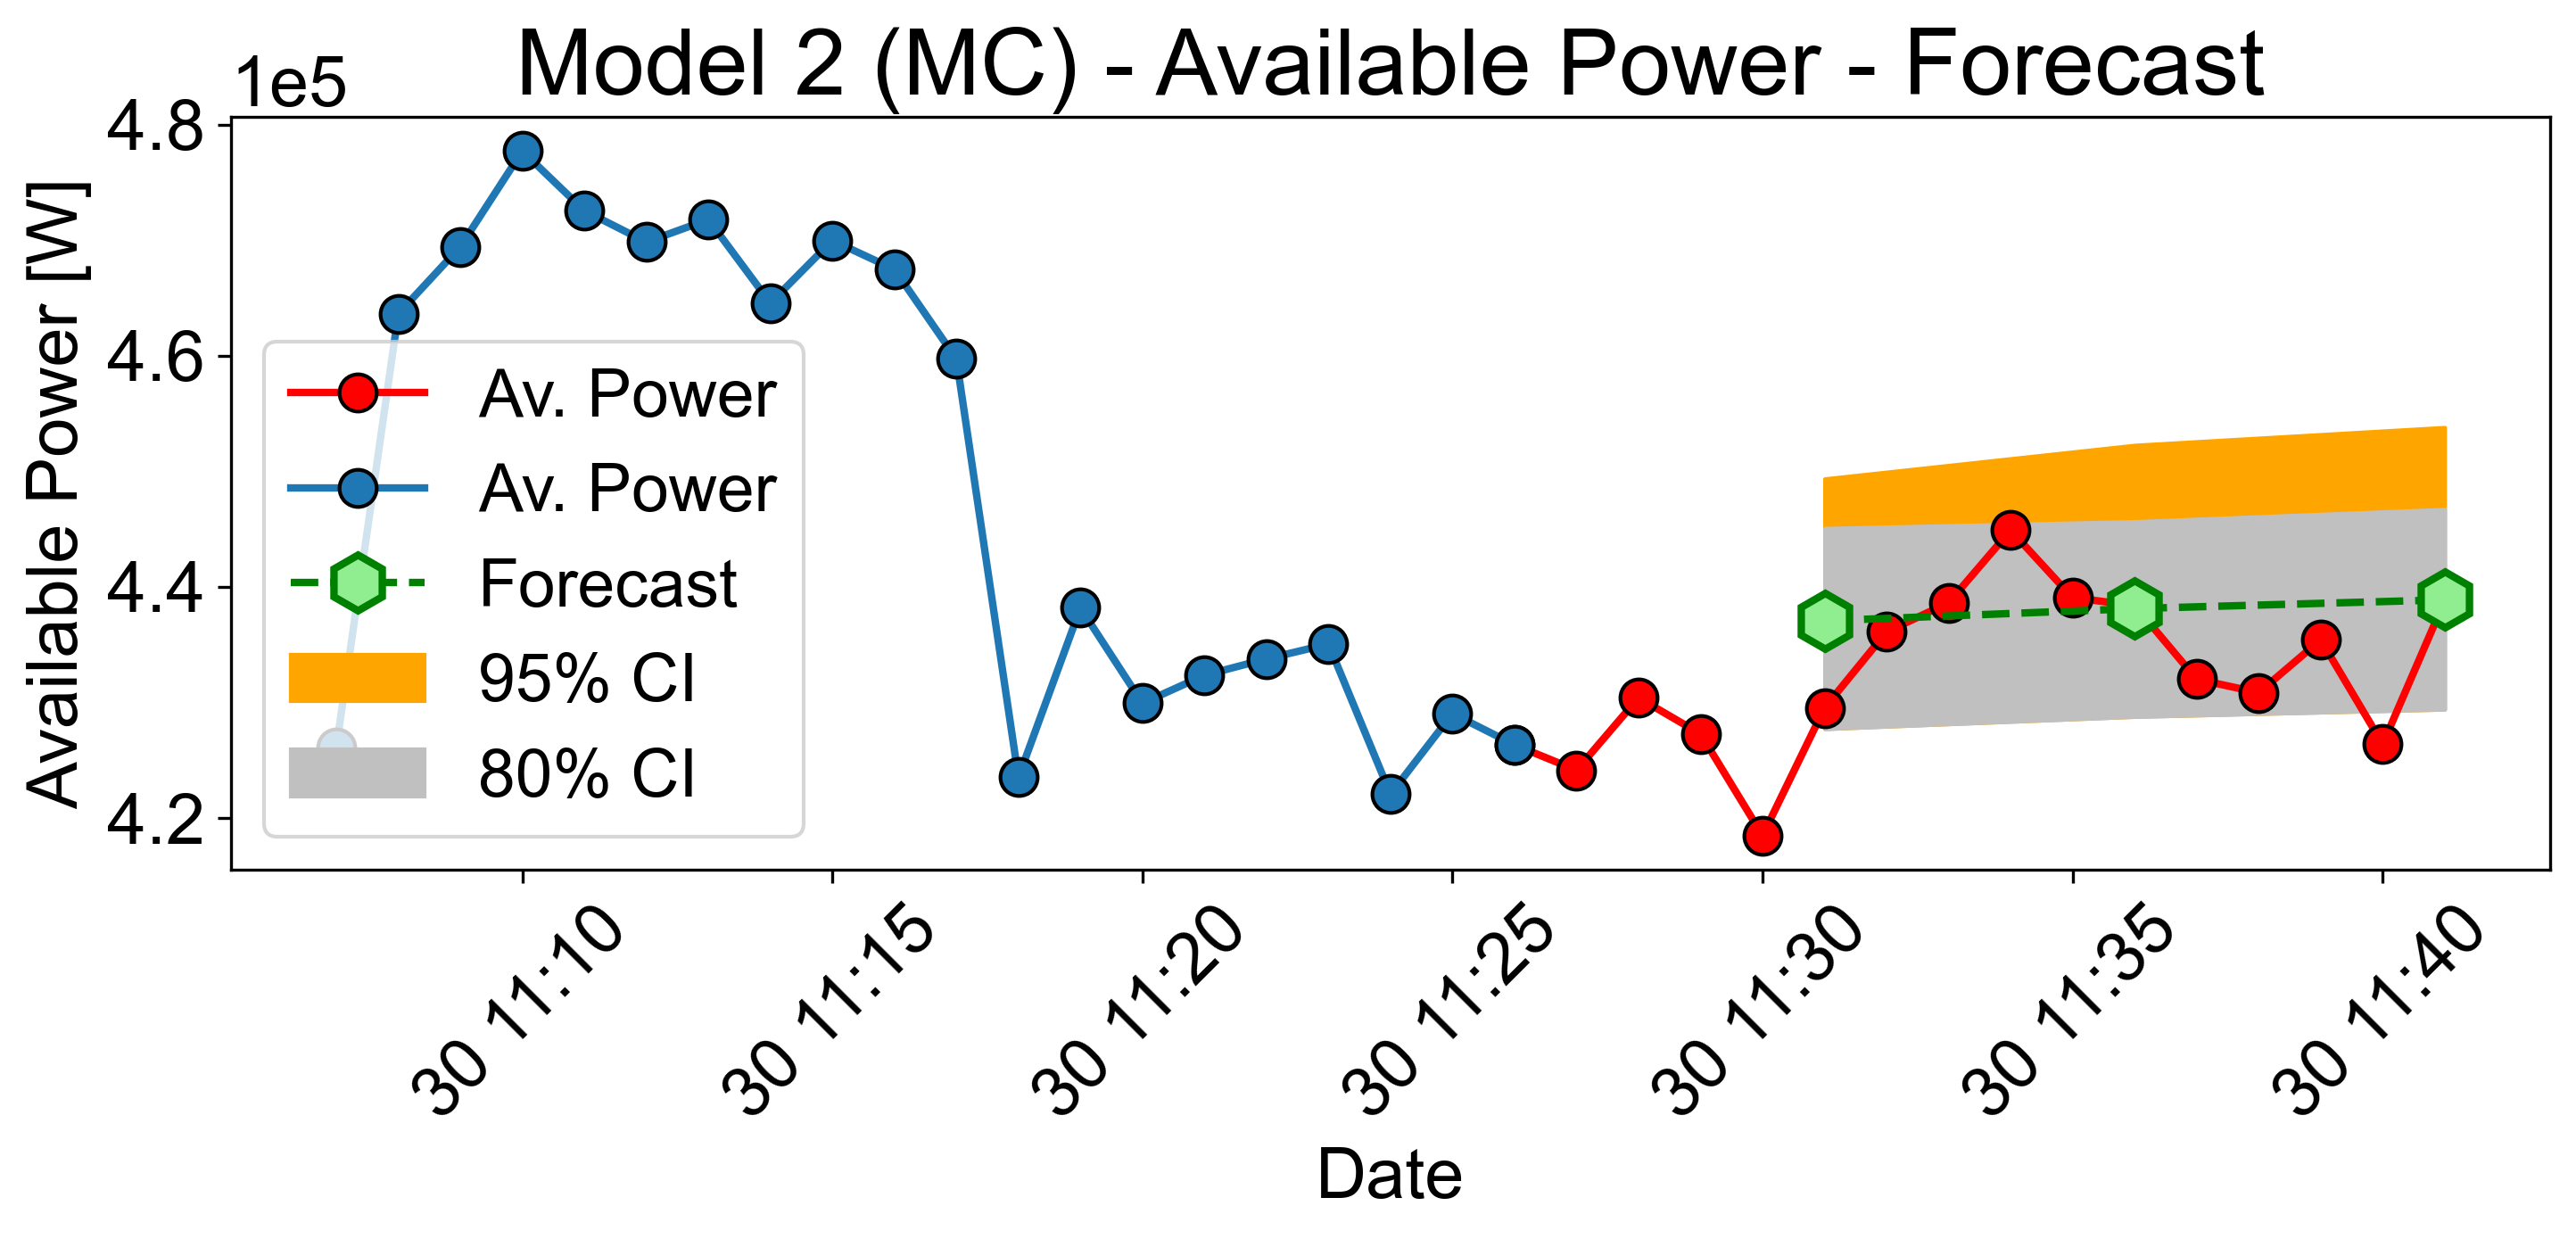
\includegraphics[width=.49\linewidth]{Images/MC-F2-LSTM-16.png}}

\subcaptionbox{\label{mc3}}{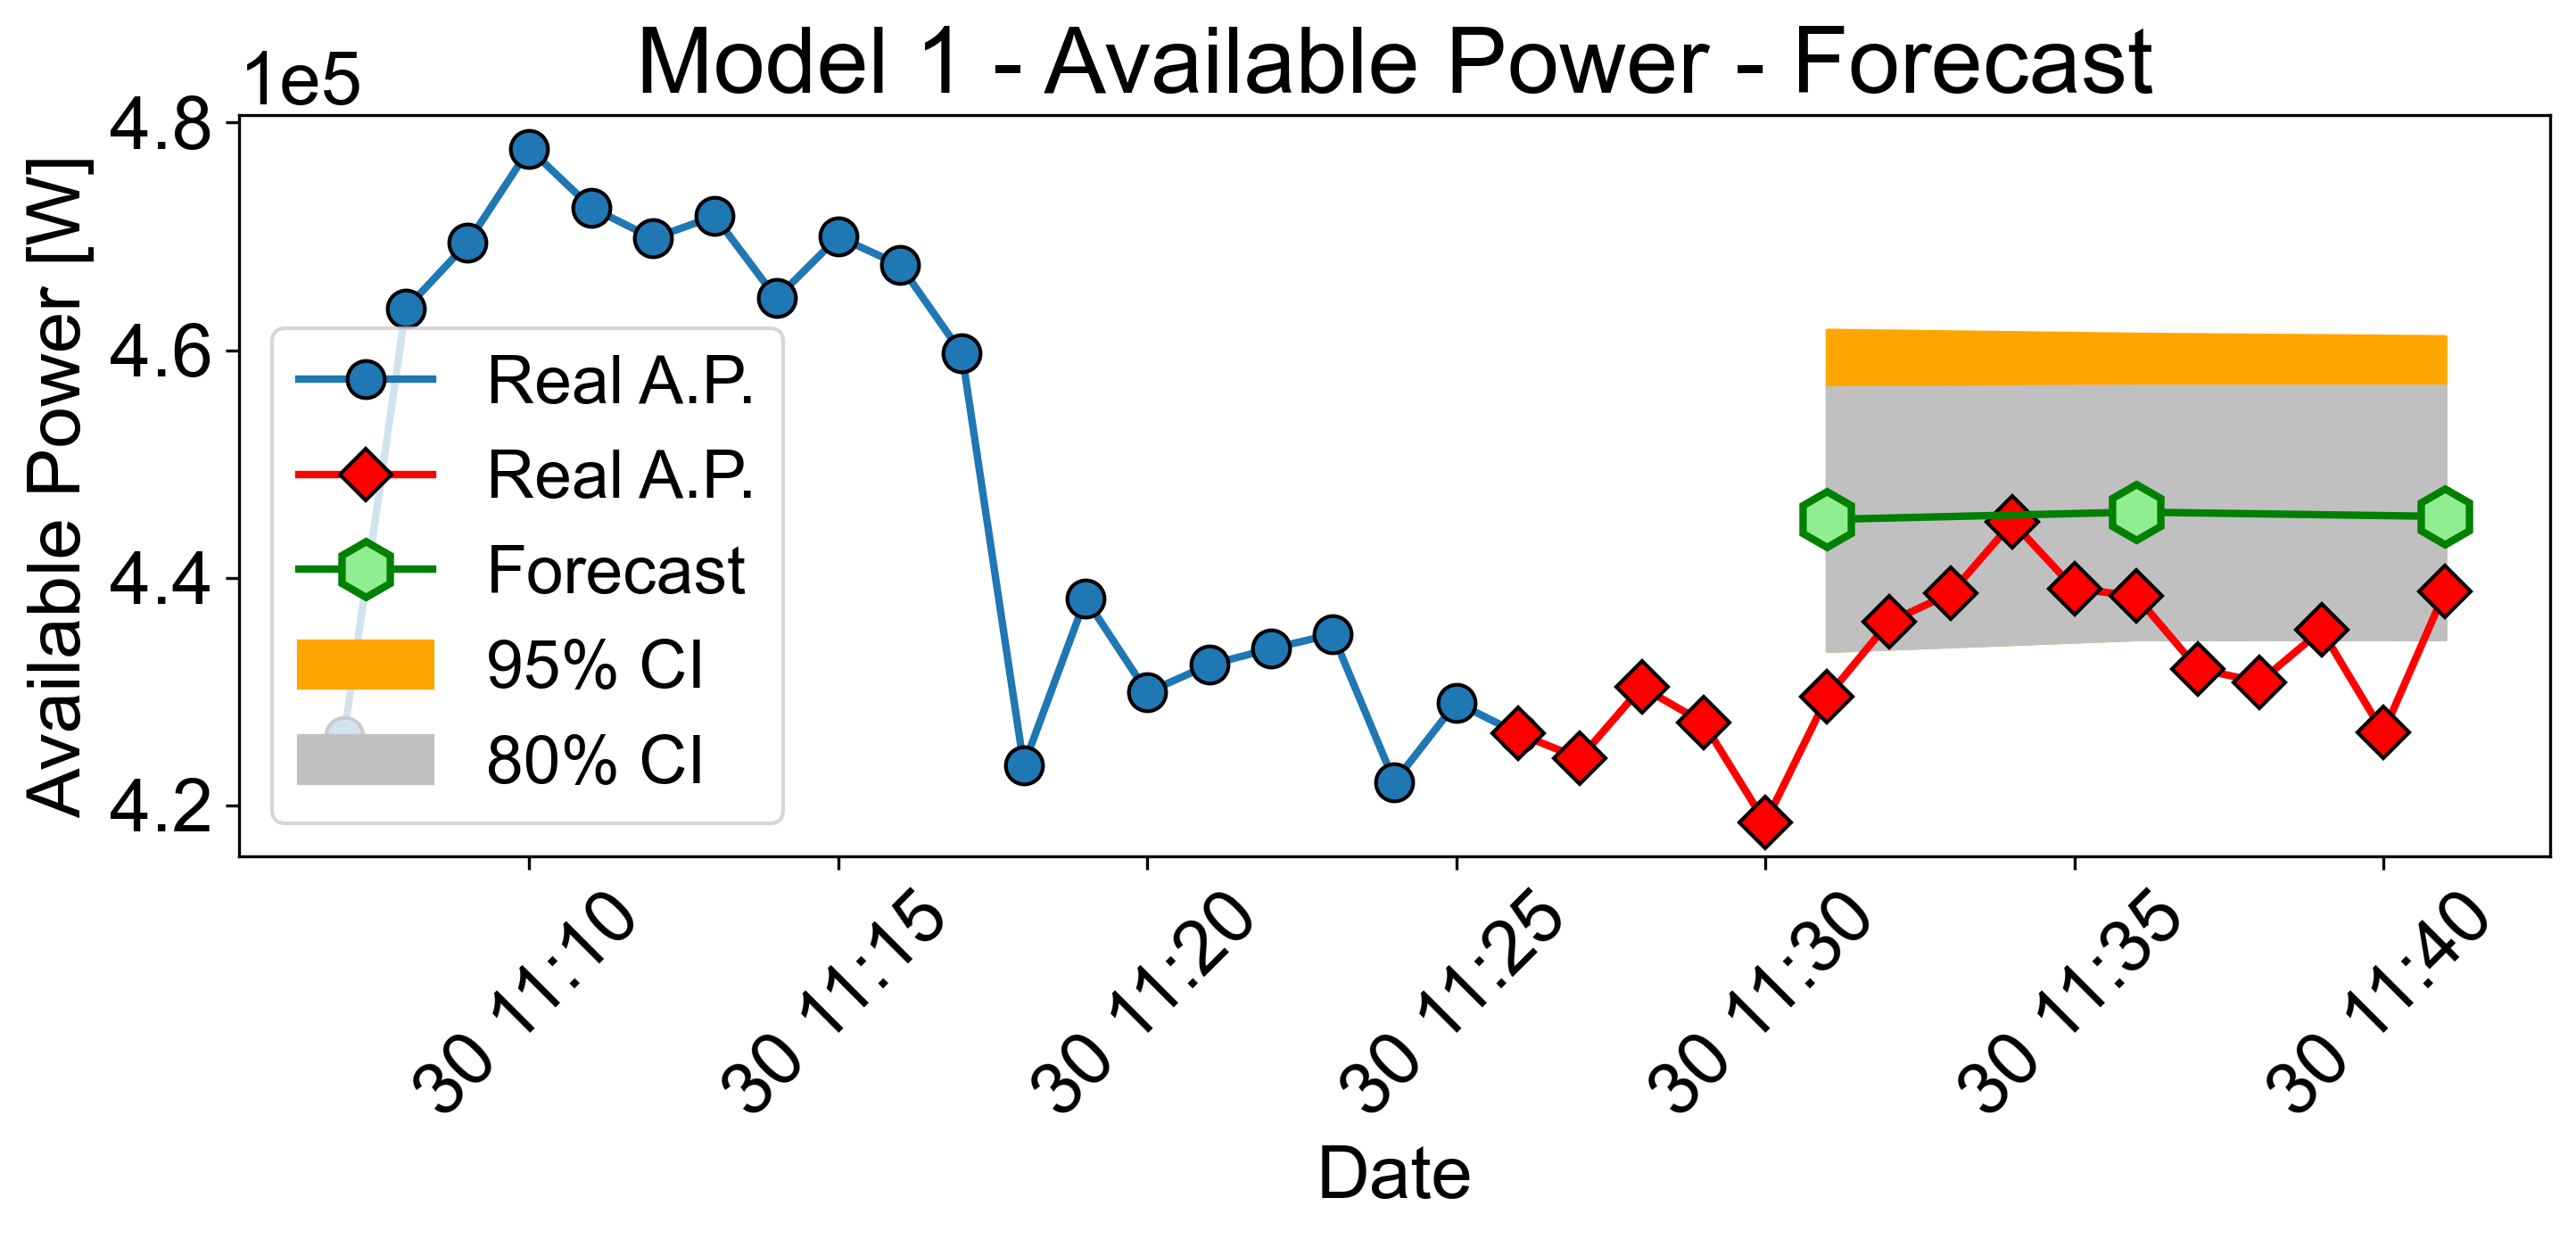
\includegraphics[width=.49\linewidth]{Images/aa.png}}
\subcaptionbox{\label{mc4}}{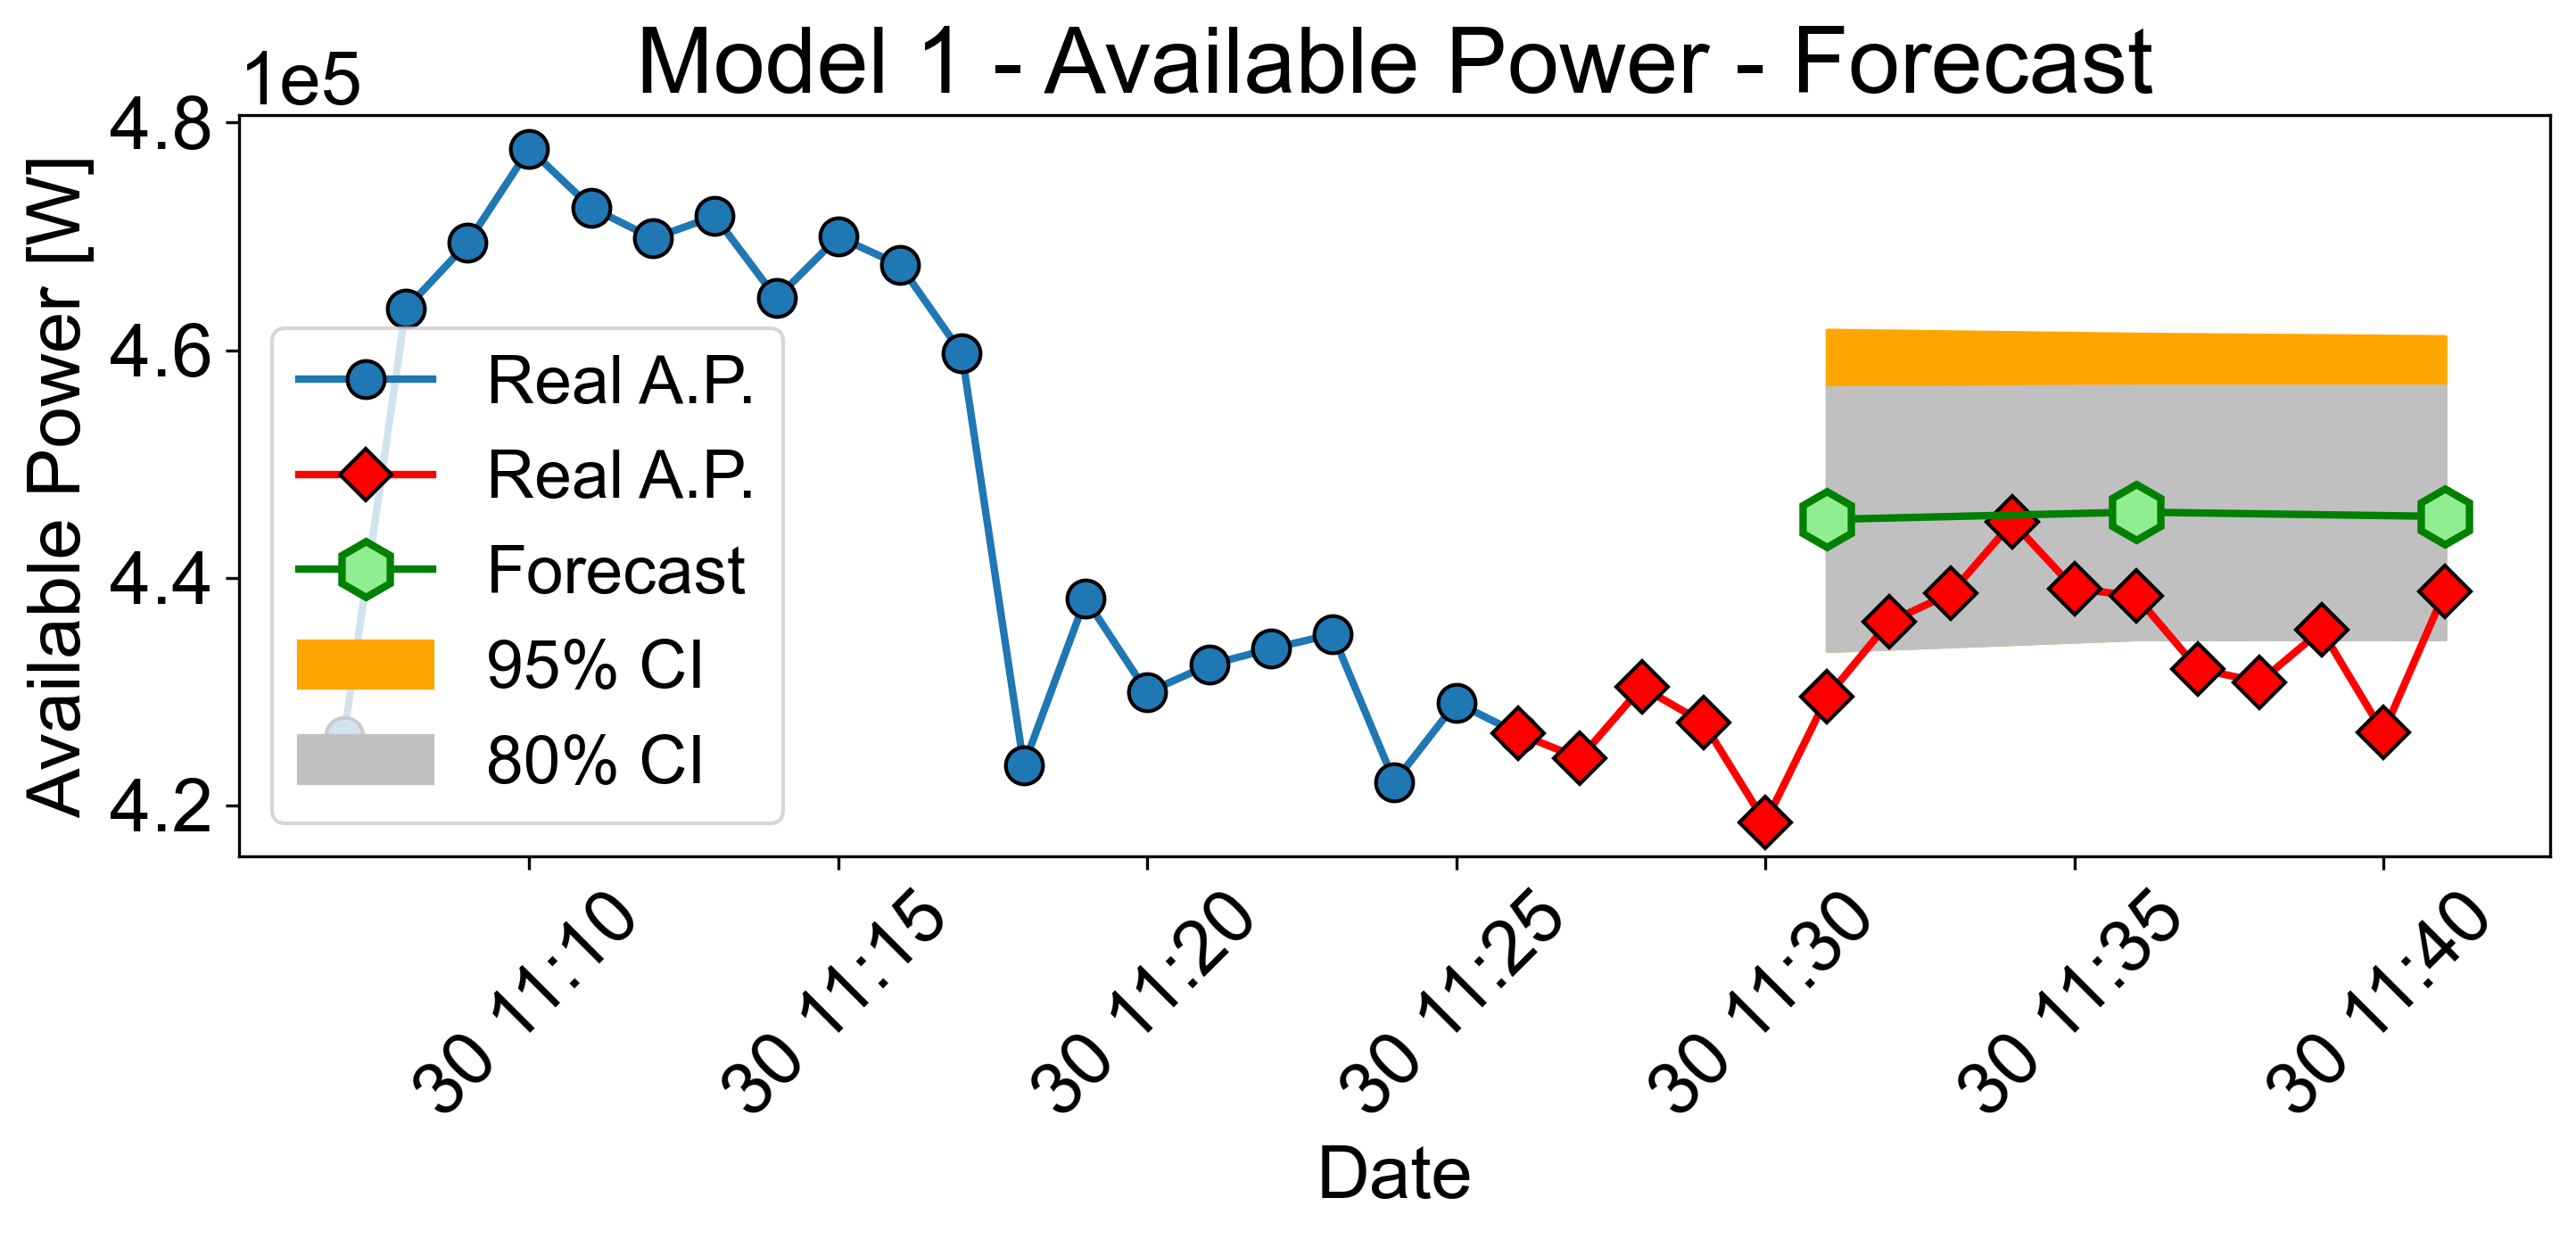
\includegraphics[width=.49\linewidth]{Images/aa.png}}

\subcaptionbox{\label{mc5}}{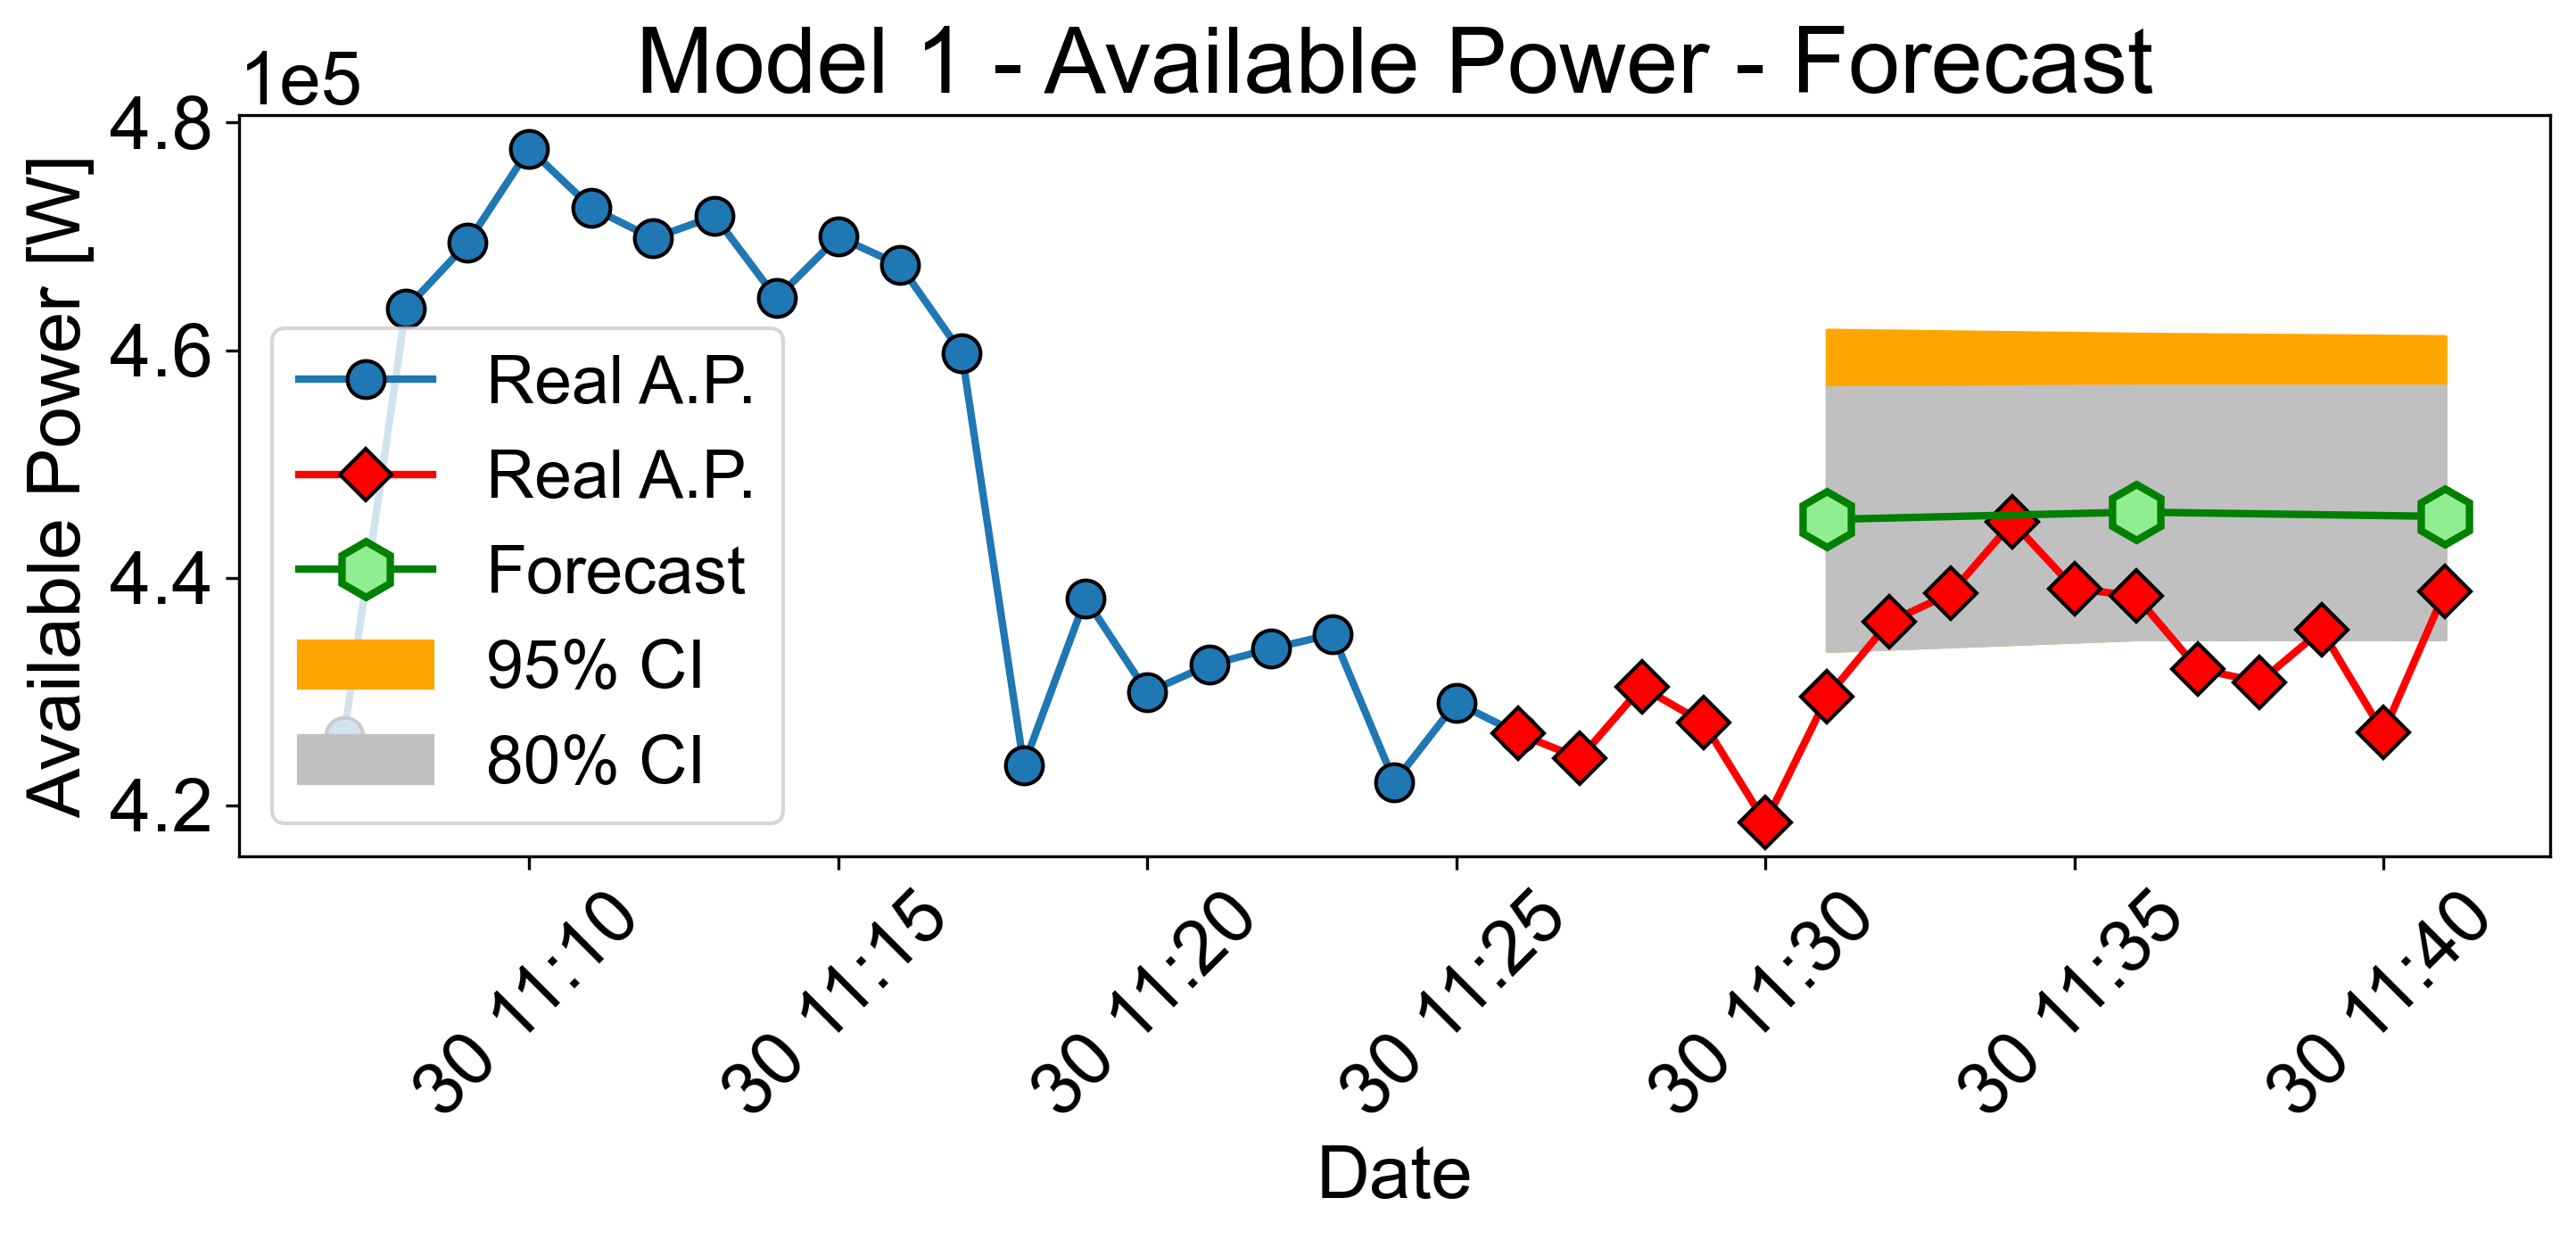
\includegraphics[width=.49\linewidth]{Images/aa.png}}
\subcaptionbox{\label{mc6}}{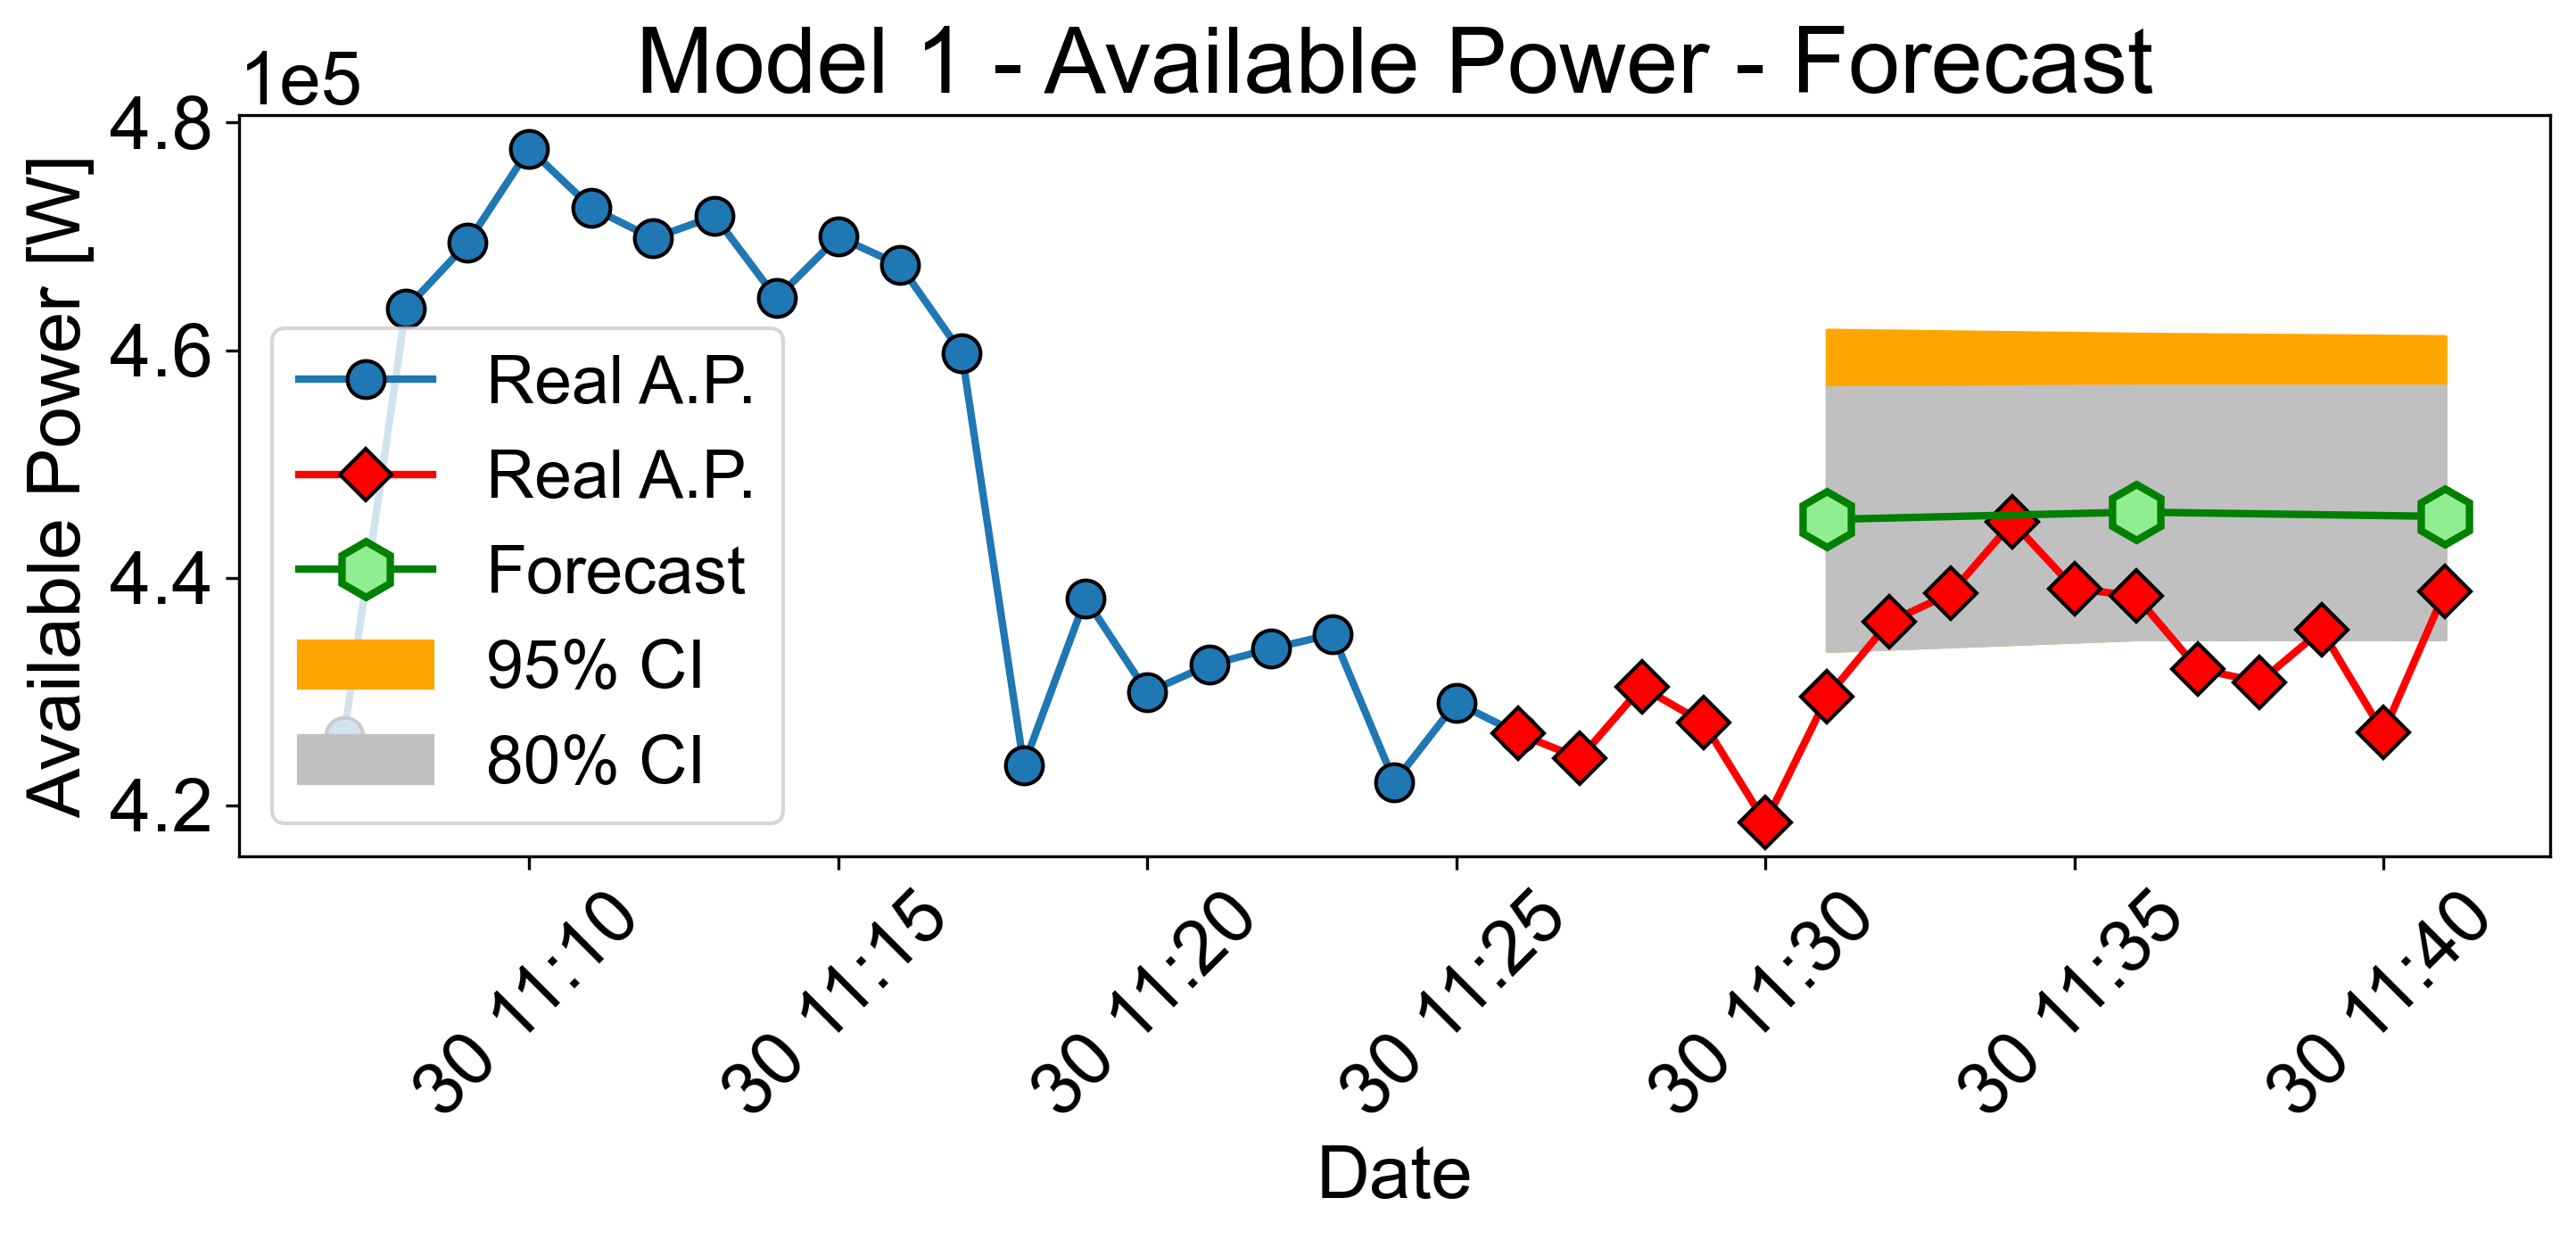
\includegraphics[width=.49\linewidth]{Images/aa.png}}
\caption{Example data a) Before convolution b) after convolution c) after Max pooling.}
\label{mtcdrop}
\end{figure}


Another issue to consider is that in the standard model, which applies dropout only in the training process, only one forecast sequence is produced, which can be called Standard Dropout Forecast. In the case where a dropout is applied in the training process and MC Dropout in the test process, a set of $N$ sequences, defined by the user, is obtained. The forecast produced in this second case is an average of the $N$ sequences produced, which can be called MC Dropout Forecast. It would be intuitive to assume that MC Dropout Forecast, since it is computed based on a set of different $N$ tests, presents a more robust estimate for the predicted values. However, the experiment was performed, where each of the 6 finalist architectures tested, for the case where it features Standard Dropout, and for the case where it features MC Dropout. The results obtained can be confirmed in Table xxx. 

\begin{table}[htbp]
  \centering
  \caption{Add caption}
    \begin{tabular}{r|cc|cccc}
    \multicolumn{1}{c|}{\multirow{2}[1]{*}{\textbf{Model}}} & \multicolumn{2}{c|}{\textbf{Vanilla}} & \multicolumn{4}{c}{\textbf{Encoder-Decoder}} \\
      & GRU & LSTM & GRU-GRU & LSTM-LSTM & CNN-GRU & CNN-LSTM \\
    \midrule
    \textbf{Test (t+5)} &   &   &   &   &   &  \\
    RMSE (E-02) & 2.521 & 2.762 & 2.606 & 2.575 & 2.694 & 3.475 \\
    RMSE MC (E-02) & 2.553 & 2.553 & 3.618 & 2.790 & 2.813 & 3.227 \\
    \textbf{Test (t+10)} &   &   &   &   &   &  \\
    RMSE (E-02) & 2.955 & 3.187 & 3.007 & 3.013 & 3.077 & 3.860 \\
    RMSE MC (E-02) & 3.049 & 2.969 & 3.908 & 3.185 & 3.196 & 3.548 \\
    \textbf{Test (t+15)} &   &   &   &   &   &  \\
    RMSE (E-02) & 3.176 & 3.344 & 3.283 & 3.308 & 3.380 & 4.106 \\
    RMSE MC (E-02) & 3.239 & 3.190 & 4.142 & 3.465 & 3.530 & 3.815 \\
    \midrule
    \textbf{Total Test} &   &   &   &   &   &  \\
    RMSE (E-02) & 2.884 & 3.098 & 2.965 & 2.965 & 3.051 & 3.814 \\
    RMSE MC (E-02) & 2.947 & 2.904 & 3.889 & 3.147 & 3.180 & 3.530 \\
    \end{tabular}%
  \label{tab:addlabel}%
\end{table}%




COMMENTS.

Although the results obtained for models with MC Dropout present a lower \ac{RMSE} value, it should be remembered that the forecasts resulting from the application of Standard Dropout are generated with a single iteration of the forecast process, while the models that apply MC Dropout result from N iterations. The more iterations carried out, the more accurate the stipulated interval will be, however the forecasting process will also take longer. It is then necessary to balance the value of $N$ with the time that $N$ iterations take to be processed. In very short-term forecasting models, as is the case, this factor is preponderant since the granularity of the data is very high and the forecasts should be immediate. It is also a factor that is directly linked to the available computing capacity.


